\begin{refsection}


\chapter{Supplements to Chapter 7}\label{appendix:a7}




\section{Computational method for \ce{Cr2O2+}}


\ce{Cr2O2+} is the smallest cluster studied in this work, but not the simplest to understand.  No single isomer obtained with the \acrshort{dft} calculations could reproduce the experimental infrared spectrum of \ce{Cr2O2+}. Therefore, as benchmark for the \acrshort{dft} optimizations, the potential hypersurface of \ce{Cr2O2+} was probed at a more accurate multireference level of theory. After crossing out geometrical structures with high relative energies based on \acrshort{dft} optimizations, the geometries of the energetically preferred structures were optimized with the multiconfigurational second-order perturbation theory restricted active space (\acrshort{raspt2}) method.\cite{raspt2} Second-order pertubative energies are obtained on the basis of the restricted active space self-consistent field (\acrshort{rasscf}) wave functions. This was done in conjunction with the \acrshort{ano}-RCC basis sets that are specifically designed for this method. The pre-defined coordinate systems for different \ce{Cr2O2+} isomers are shown in Figure \ref{a7fig:Cr2O2-coord}. 

All \acrshort{rasscf} wave functions were generated from the distribution of 19 electrons in 18 active orbitals (6 in RAS1, 12 in RAS2 and 0 in RAS3), in which the maximum number of electrons excited from RAS1 is 2. The short term for this calculation can be written as RAS(19,2,0;6,12,0). All 3p orbitals of two oxygen atoms are correlated in RAS1, while RAS2 chiefly contains the 4s and 3d orbitals of the two chromium atoms. By optimizing with the double-$\zeta$ basis set \acrshort{ano}-RCC-VDZ,\cite{ano-basisnm, ano-basisM} a few lowest states with specific spins were selected and reoptimized with the quadruple-$\zeta$ basis set \acrshort{ano}-RCC-VQZP.\cite{ano-basisnm, ano-basisM} The dynamic correlation energy was treated by second-order perturbation without inclusion of core orbitals from chromium and oxygen (1s of oxygen, 3p and inner subshell orbitals of chromium). All \acrshort{rasscf}/\acrshort{raspt2} calculations were performed with MOLCAS 8.1.\cite{molcas81}

\begin{figure}[htbp!]
    \centering
	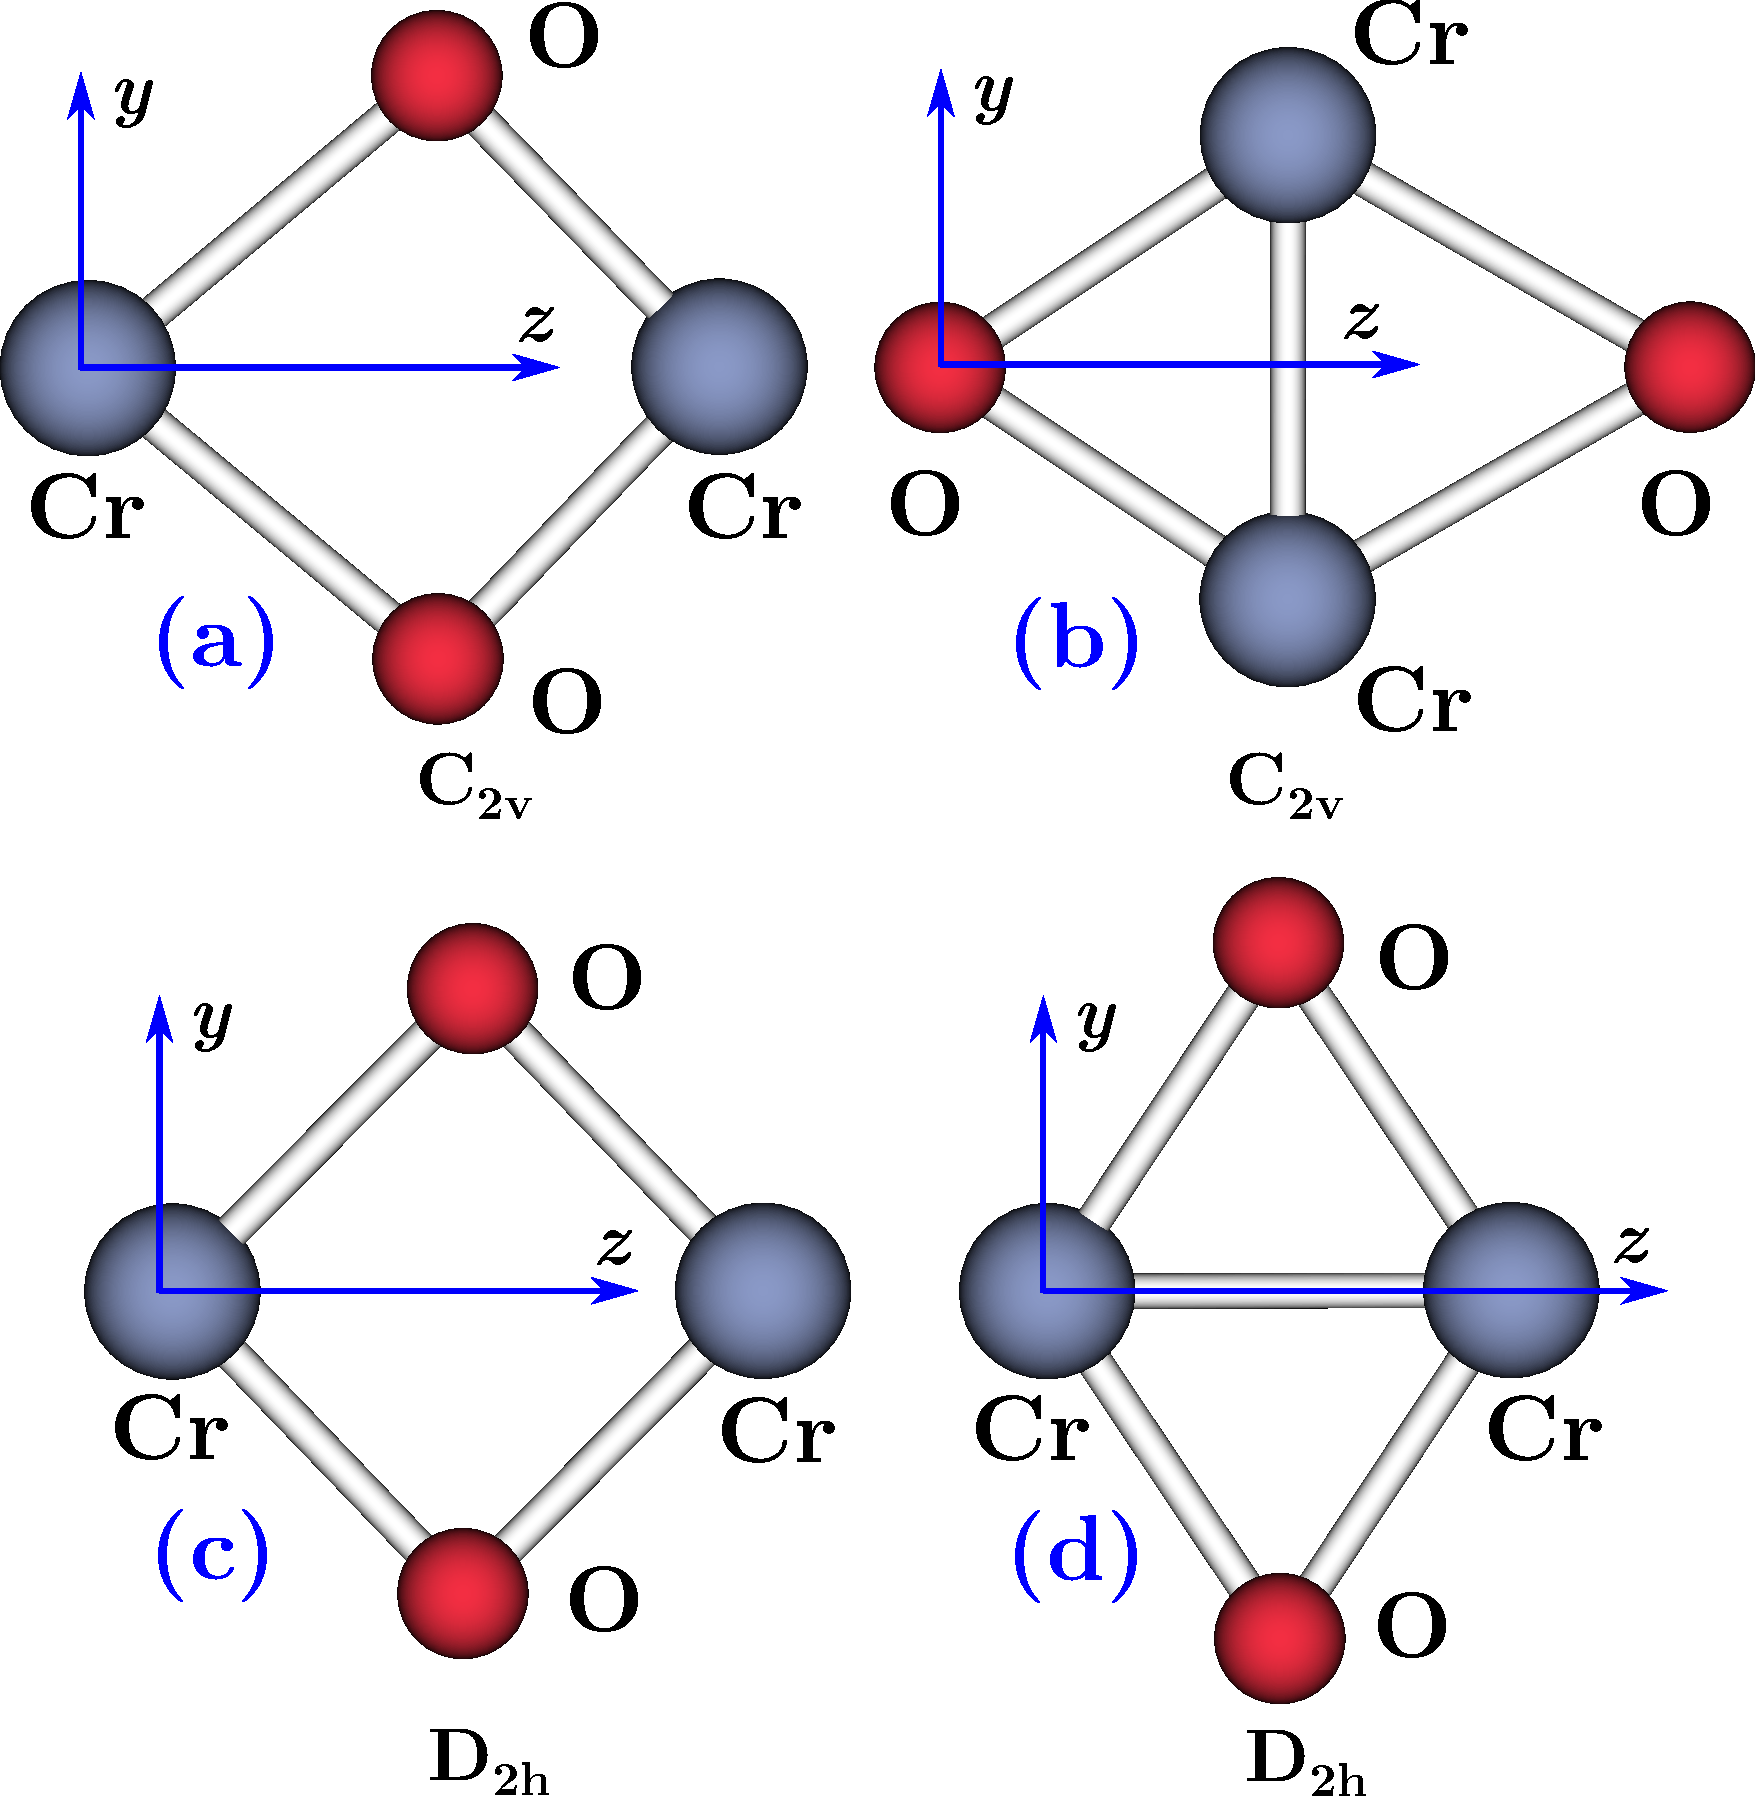
\includegraphics[width=0.8\textwidth]{Cr2O2-coord}
	\caption{Coordinate systems used for the \acrshort{rasscf}/\acrshort{raspt2} calculations of three initial structures of \ce{Cr_2O_2^+}. After optimization, the structures converged to the D$_{2h}$ point group on left.}
	\label{a7fig:Cr2O2-coord}
\end{figure}

Starting from the electronic structures obtained from the \acrshort{rasscf} calculations, we reoptimized the geometries of some of the lowest states at different \acrshort{dft} levels (B3LYP,\cite{lyp, b3lyp2, b3} B3P86,\cite{b3,p86} B3PW91,\cite{b3} BP86,\cite{b3lyp2, p86} TPSS,\cite{tpss} TPSSh, and M06L\cite{m06l}). Furthermore, single-point energies at the restricted coupled cluster single-double and perturbative triple (\acrshort{rccsd}(T)-F12) level were also computed making use of the \acrshort{raspt2} optimal geometries. These additional calculations ensured identification of the ground state and the first excited state. All \acrshort{dft} calculations were done in conjunction with the correlation-consistent polarized basis set cc-pVTZ.\cite{basis-augM,basis-ccO} At the \acrshort{rccsd}(T)-F12 level,\cite{f12.1,f12.2} the aug-cc-pVTZ\cite{basis-augM} for Cr and cc-pVTZ-F12\cite{basis-F12} for oxygen were used. Unless otherwise noted, all calculations are done with the Molpro 2012.1 package.\cite{molpro2012} All electron scalar relativistic effects were taken into account by the second-order Douglas-Kroll-Hess Hamiltonian (DKH2)\cite{DKH} for all \ce{Cr2O2+} calculations. The correlation energy from \acrshort{rccsd}(T)-F12 was recovered without consideration of core orbitals as mentioned above for \acrshort{raspt2} calculations. Because of the technical shortcomings of the used programs, \acrshort{zpe}s of all considered states cannot be obtained; therefore, relative energies of \ce{Cr2O2+} states at \acrshort{dft}, \acrshort{rccsd}(T)-F12 and \acrshort{raspt2} levels were calculated from bare electronic values. For those small clusters, \acrshort{zpe}s are expected to insignificantly affect relative energies of different states.\cite{ZPE}

\newpage

\section[Relative Energies]{Relative Energies of Different Electronic States of \ce{Cr2O2+}}

Table \ref{a7tbl:Cr2O2} contains the relative energies of different electronic states of \ce{Cr2O2+} at different computational levels. The energies were calculated with the Molpro 2015.1 package, except for the B3P86 and B3PW91, which were calculated using the Gaussian 09 code  and the \acrshort{ccsd}(T)-F12 energy values were computed with Molpro 2012.1.  

\begin{table}[!htbp]
    \centering
    \small
	\caption{Relative energies (in eV) of the low-lying electronic states of \ce{Cr2O2+} at the several levels of theory}
	\label{a7tbl:Cr2O2}
	\begin{threeparttable}
	\begin{tabular}{lrrrrrrrrr}
		\hline
		\multirow{2}{*}{states} & \multicolumn{9}{c}{method}                                          				   \\ \cline{2-10} 
				& TPSS 	 & B3P86\tnote{a}   & B3LYP & B3PW91\tnote{a}   & BP86 & M06L & TPSSh & F12a\tnote{b} & \acrshort{raspt2} \\ \hline
$^8$B$_{1g}$    & 0.00   & 0.00  			& 0.00  & 0.00   			& 0.00 & 0.00 & 0.00  & 0.00 		  & 0.00   \\
$^8$B$_{1u}$    & 0.58   & 0.46  			& 0.51  & 0.46   			& 0.45 & 0.45 & 0.55  & 0.45 		  & 0.38   \\
$^8$A$_g$       & 0.64   &       			& 0.56  &        			& 0.60 & 0.57 & 0.63  & 0.58 		  & 0.52   \\
$^8$B$_{3u}$    & 0.61   &       			& 0.68  &        			& 0.60 & 0.62 & 0.65  & 0.67 		  & 0.89   \\
$^8$B$_{2u}$    & 1.64   &       			& 1.50  &        			& 1.56 & 1.57 & 1.64  & 1.44 		  & 1.38   \\
$^8$B$_{2g}$    & 1.37   &       			& 1.55  &        			& 1.52 & 1.52 & 1.49  & 1.38 		  & 1.39   \\
$^8$B$_{3g}$    & 1.91   &       			& 2.45  &        			& 2.01 & 2.00 & 2.23  & 2.17 		  & 2.65   \\
$^8$A$_{u}$     & 1.59   &       			& 1.79  &        			& 1.71 & 1.71 & 1.73  & 1.50 		  & 1.58   \\ \hline
	\end{tabular}
	  \begin{tablenotes}
		\item[a]These energies are calculated with Gaussian 09.
		\item[b]F12a is an abbreviation for \acrshort{rccsd}(T)-F12a.
	\end{tablenotes}
\end{threeparttable}
\end{table}


\begin{table}[]
	\centering
	\caption{CASSCF pseudonatural leading configurations of the low-lying energetic states of \ce{Cr2O2+}}
	\label{a7tbl:leadconfg}
	\begin{tabular}{lr}
		\hline
		state  & \multicolumn{1}{c}{leading configuration}                                                                \\ \hline
 $^8$B$_{1g}$  & 9a$_g^1$ 10a$_g^1$ 3b$_{3u}^2$ 4b$_{3u}^1$ 5b$_{2u}^2$ 1b$_{1g}^2$ 2b$_{1g}^0$ 6b$_{1u}^2$ 7b$_{1u}^1$ 8b$_{1u}^1$ 3b$_{2g}^1$ 3b$_{3g}^2$ 4b$_{3g}^0$ 1a$_u^1$ \\
 $^8$B$_{1u}$  & 9a$_g^1$ 10a$_g^1$ 3b$_{3u}^2$ 4b$_{3u}^1$ 5b$_{2u}^2$ 1b$_{1g}^2$ 2b$_{1g}^1$ 6b$_{1u}^2$ 7b$_{1u}^0$ 8b$_{1u}^1$ 3b$_{2g}^1$ 3b$_{3g}^2$ 4b$_{3g}^0$ 1a$_u^1$ \\
 $^8$A$_{g }$  & 9a$_g^0$ 10a$_g^1$ 3b$_{3u}^2$ 4b$_{3u}^1$ 5b$_{2u}^2$ 1b$_{1g}^2$ 2b$_{1g}^1$ 6b$_{1u}^2$ 7b$_{1u}^1$ 8b$_{1u}^1$ 3b$_{2g}^1$ 3b$_{3g}^2$ 4b$_{3g}^0$ 1a$_u^1$ \\
 $^8$B$_{3u}$  & 9a$_g^1$ 10a$_g^1$ 3b$_{3u}^2$ 4b$_{3u}^0$ 5b$_{2u}^2$ 1b$_{1g}^2$ 2b$_{1g}^1$ 6b$_{1u}^2$ 7b$_{1u}^1$ 8b$_{1u}^1$ 3b$_{2g}^1$ 3b$_{3g}^2$ 4b$_{3g}^0$ 1a$_u^1$ \\
 $^8$B$_{2u}$  & 9a$_g^0$ 10a$_g^1$ 3b$_{3u}^2$ 4b$_{3u}^1$ 5b$_{2u}^2$ 1b$_{1g}^2$ 2b$_{1g}^1$ 6b$_{1u}^2$ 7b$_{1u}^0$ 8b$_{1u}^1$ 3b$_{2g}^1$ 3b$_{3g}^2$ 4b$_{3g}^1$ 1a$_u^1$ \\
 $^8$B$_{2g}$  & 9a$_g^1$ 10a$_g^1$ 3b$_{3u}^2$ 4b$_{3u}^1$ 5b$_{2u}^2$ 1b$_{1g}^2$ 2b$_{1g}^1$ 6b$_{1u}^2$ 7b$_{1u}^1$ 8b$_{1u}^1$ 3b$_{2g}^0$ 3b$_{3g}^2$ 4b$_{3g}^0$ 1a$_u^1$ \\
 $^8$B$_{3g}$  & 9a$_g^1$ 10a$_g^1$ 3b$_{3u}^2$ 4b$_{3u}^1$ 5b$_{2u}^1$ 1b$_{1g}^2$ 2b$_{1g}^0$ 6b$_{1u}^2$ 7b$_{1u}^1$ 8b$_{1u}^1$ 3b$_{2g}^1$ 3b$_{3g}^2$ 4b$_{3g}^0$ 1a$_u^2$ \\
 $^8$A$_{u}$  & 9a$_g^1$ 10a$_g^1$ 3b$_{3u}^2$ 4b$_{3u}^1$ 5b$_{2u}^2$ 1b$_{1g}^2$ 2b$_{1g}^1$ 6b$_{1u}^2$ 7b$_{1u}^1$ 8b$_{1u}^1$ 3b$_{2g}^1$ 3b$_{3g}^2$ 4b$_{3g}^0$ 1a$_u^0$ \\ \hline
	\end{tabular}
\end{table}



\newpage

\section{Influence of Messenger atoms on the \acrshort{ir} Spectra}

The effect of the attached rare gas atoms on the infrared spectra is assessed at the TPSS level for the lowest energy isomers of \ce{Cr2O2+$\boldsymbol{\cdot}$Ne}, \ce{Cr3O+$\boldsymbol{\cdot}$He2}, and \ce{Cr3O2+$\boldsymbol{\cdot}$He}. For these clusters respectively Ne, \ce{He2} and He were used as messenger. As can be seen in Figure \ref{a7fig:with-NeHe}, the influence of the messenger atoms on the infrared spectra is minor.


\begin{figure}[htb!]
	\centering
	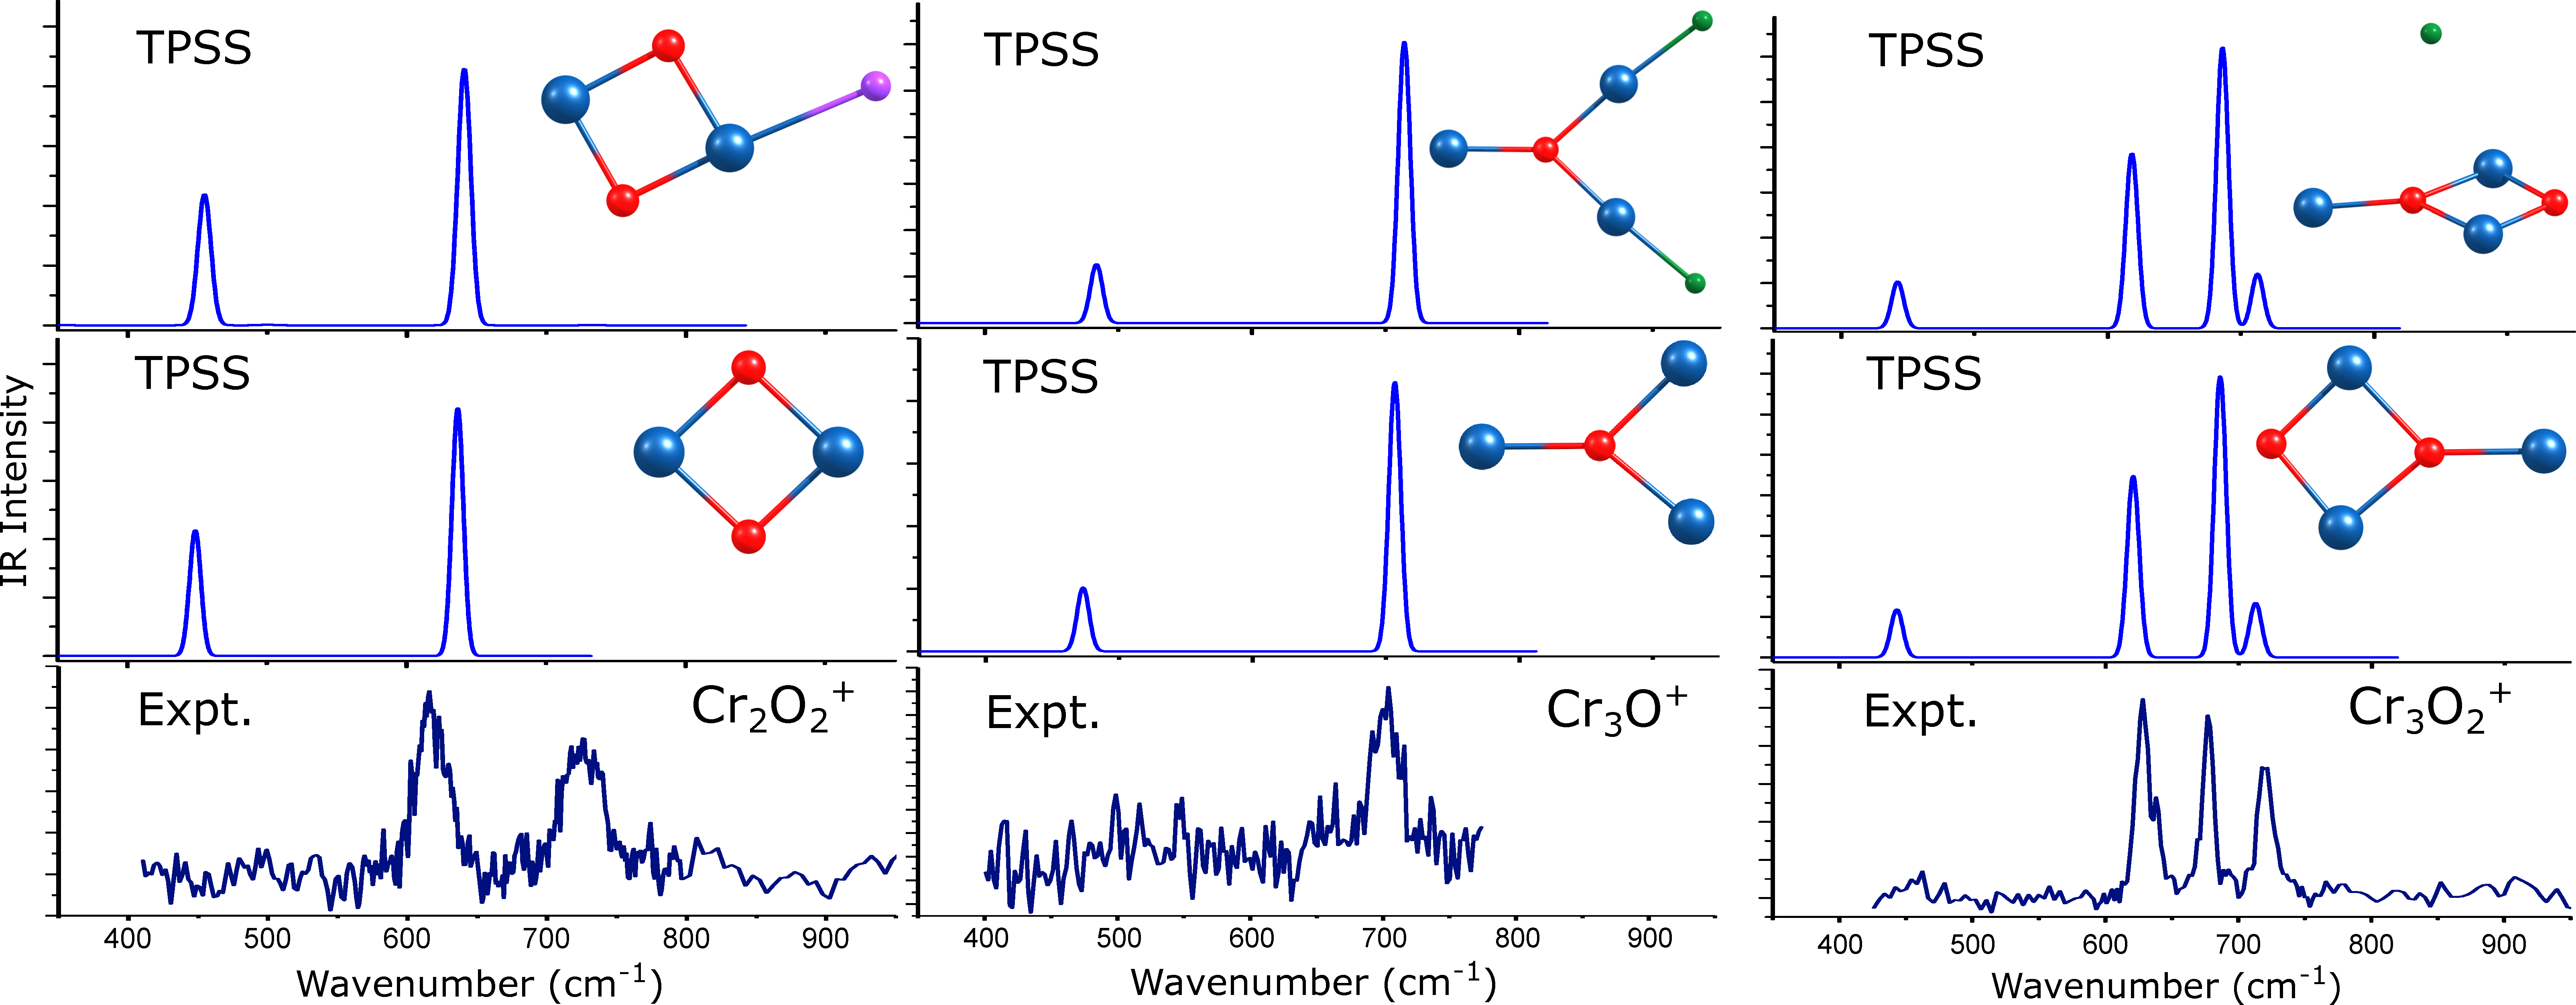
\includegraphics[width=\textwidth]{IR-with-NeHe.pdf}
	\caption{Computational assessment of the effect of rare gas attachment on the simulated infrared spectra at the TPSS level of theory. Shown are the experimental \acrshort{irpd}  spectra of \ce{Cr2O2+}$\boldsymbol{\cdot}$Ne, \ce{Cr3O+$\boldsymbol{\cdot}$He2}, and \ce{Cr3O2+$\boldsymbol{\cdot}$He} (bottom row) and the simulated spectra for the ground state structure of the bare clusters (middle row) and of the cluster-rare gas complexes (top row).}
	\label{a7fig:with-NeHe}
\end{figure}


%%%%%%%%%% Cr3O+%%%%%%%%%%

\newpage
\section[Geometric Structures of \ch{C\lowercase{r}3O_{\lowercase{m}}^+} (\lowercase{m} = 1 -- 5) and \ch{C\lowercase{r}4O4+}]{Structures of the Lowest Energy Isomers of \ch{Cr3O_{\lowercase{m}}^+} (\lowercase{m} = 1 -- 5) and \ch{Cr4O4+}}

\begin{figure}[]
	\centering
	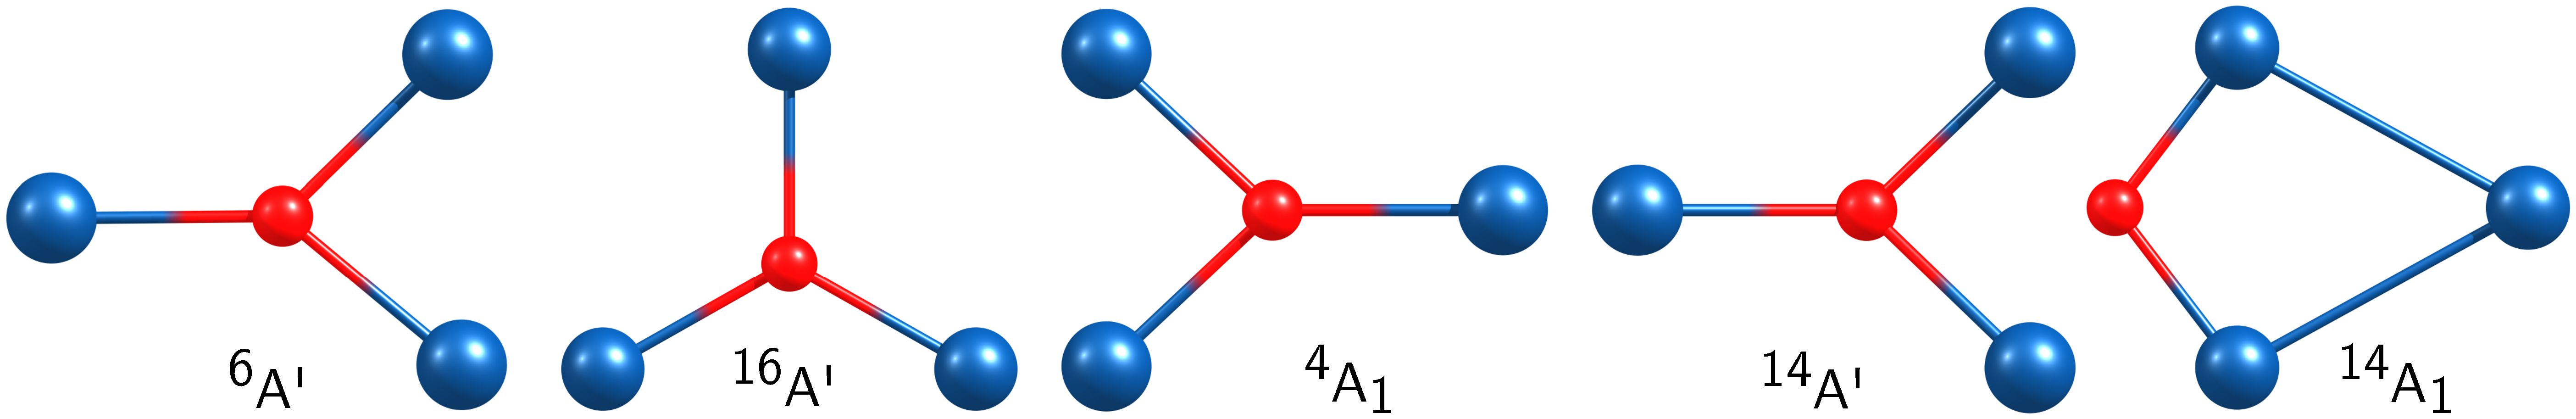
\includegraphics[width=0.85\textwidth]{Cr3O-isomers.pdf}
	\caption{Geometrical structures of the lowest energy isomers of \ce{Cr3O+}. The shown structures are obtained with the TPSS/cc-pVTZ optimizations. Chromium and oxygen atoms are represented as blue and red spheres, respectively.}
	\label{a7fig:Cr3O-isomers}
\end{figure}

\begin{figure}[]
	\centering
	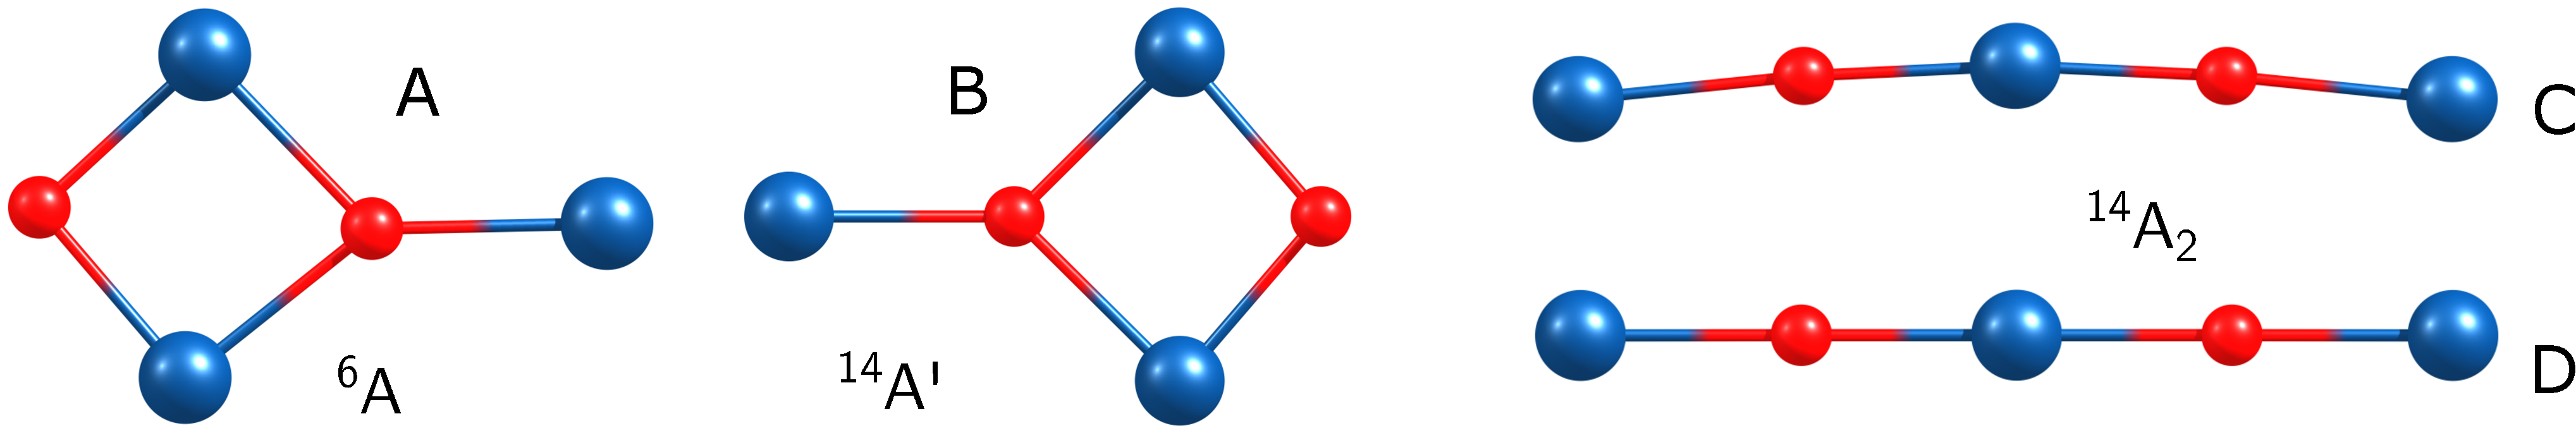
\includegraphics[width=0.85\textwidth]{Cr3O2-isomers.pdf}
	\caption{Geometrical structures of the lowest energy isomers of \ce{Cr3O2+}. The shown structures are obtained with the TPSS/cc-pVTZ optimizations, except for  isomer C, which was obtained at the B3P86/cc-pVTZ level. }
	\label{a7fig:Cr3O2-isomers}
\end{figure}

\begin{figure}[]
	\centering
	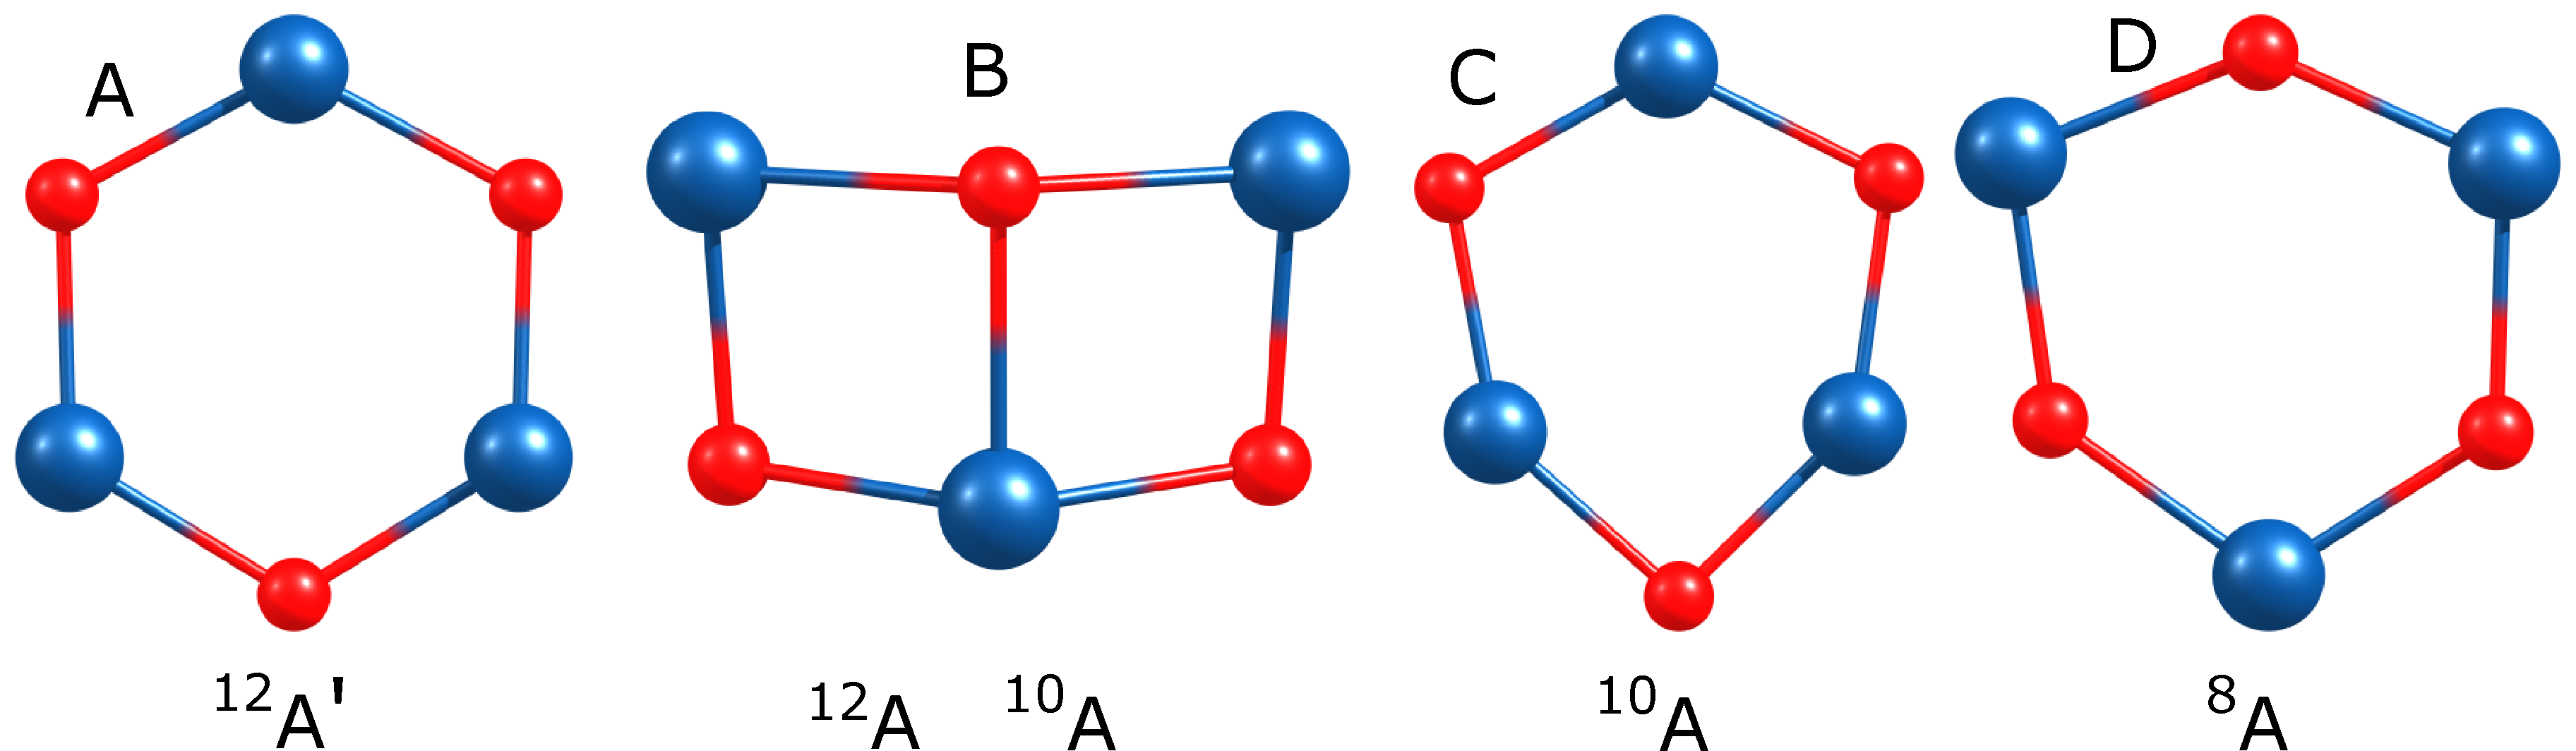
\includegraphics[width=0.7\textwidth]{Cr3O3-isomers.pdf}
	\caption{Geometrical structures of the lowest energy isomers of \ce{Cr3O3+}.}
	\label{a7fig:Cr3O3-isomers}
\end{figure}

\begin{figure}[]
	\centering
	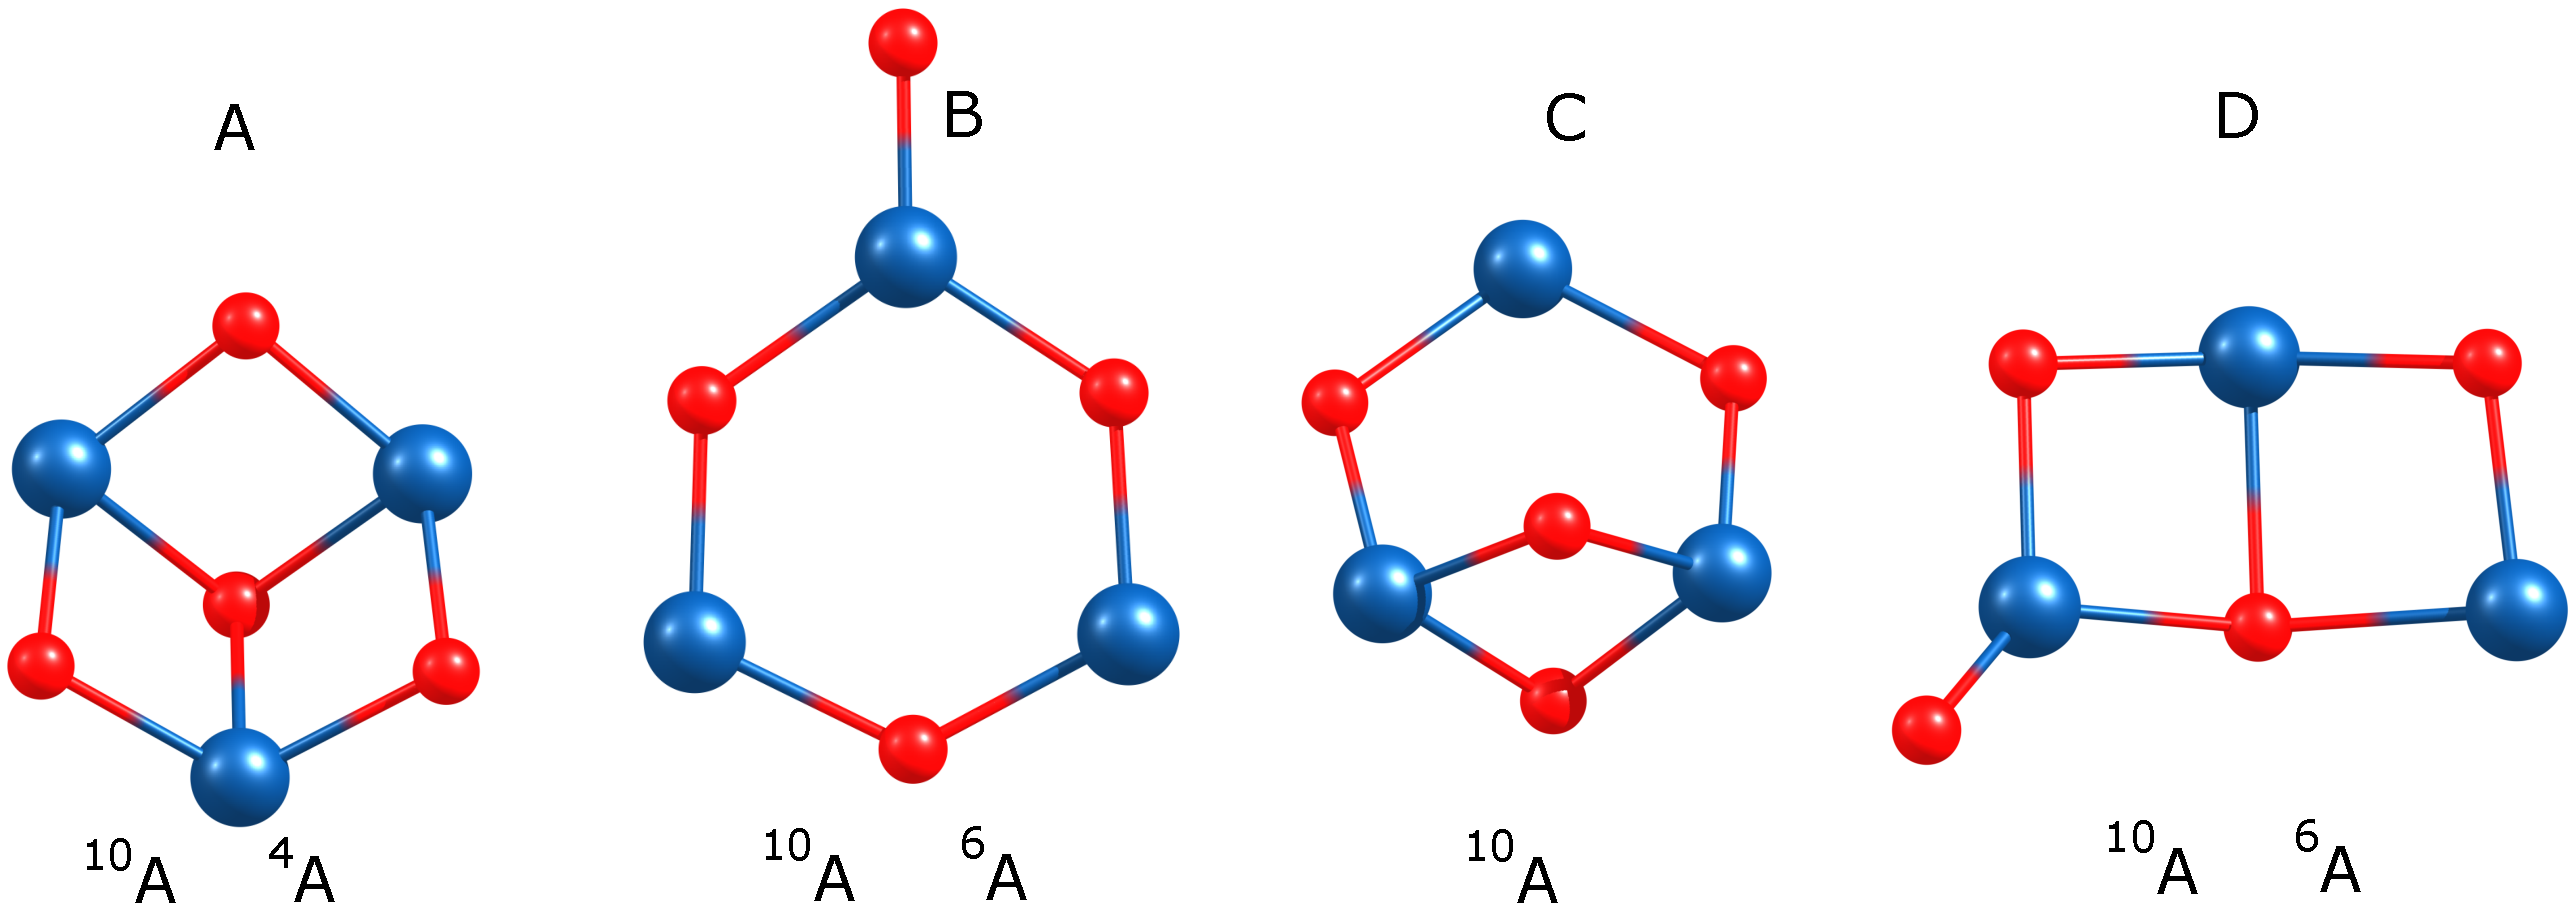
\includegraphics[width=0.8\textwidth]{Cr3O4-isomers.pdf}
	\caption{Geometrical structures of the lowest energy isomers of \ce{Cr3O4+}.}
	\label{a7fig:Cr3O4-isomers}
\end{figure}

\begin{figure}[]
	\centering
	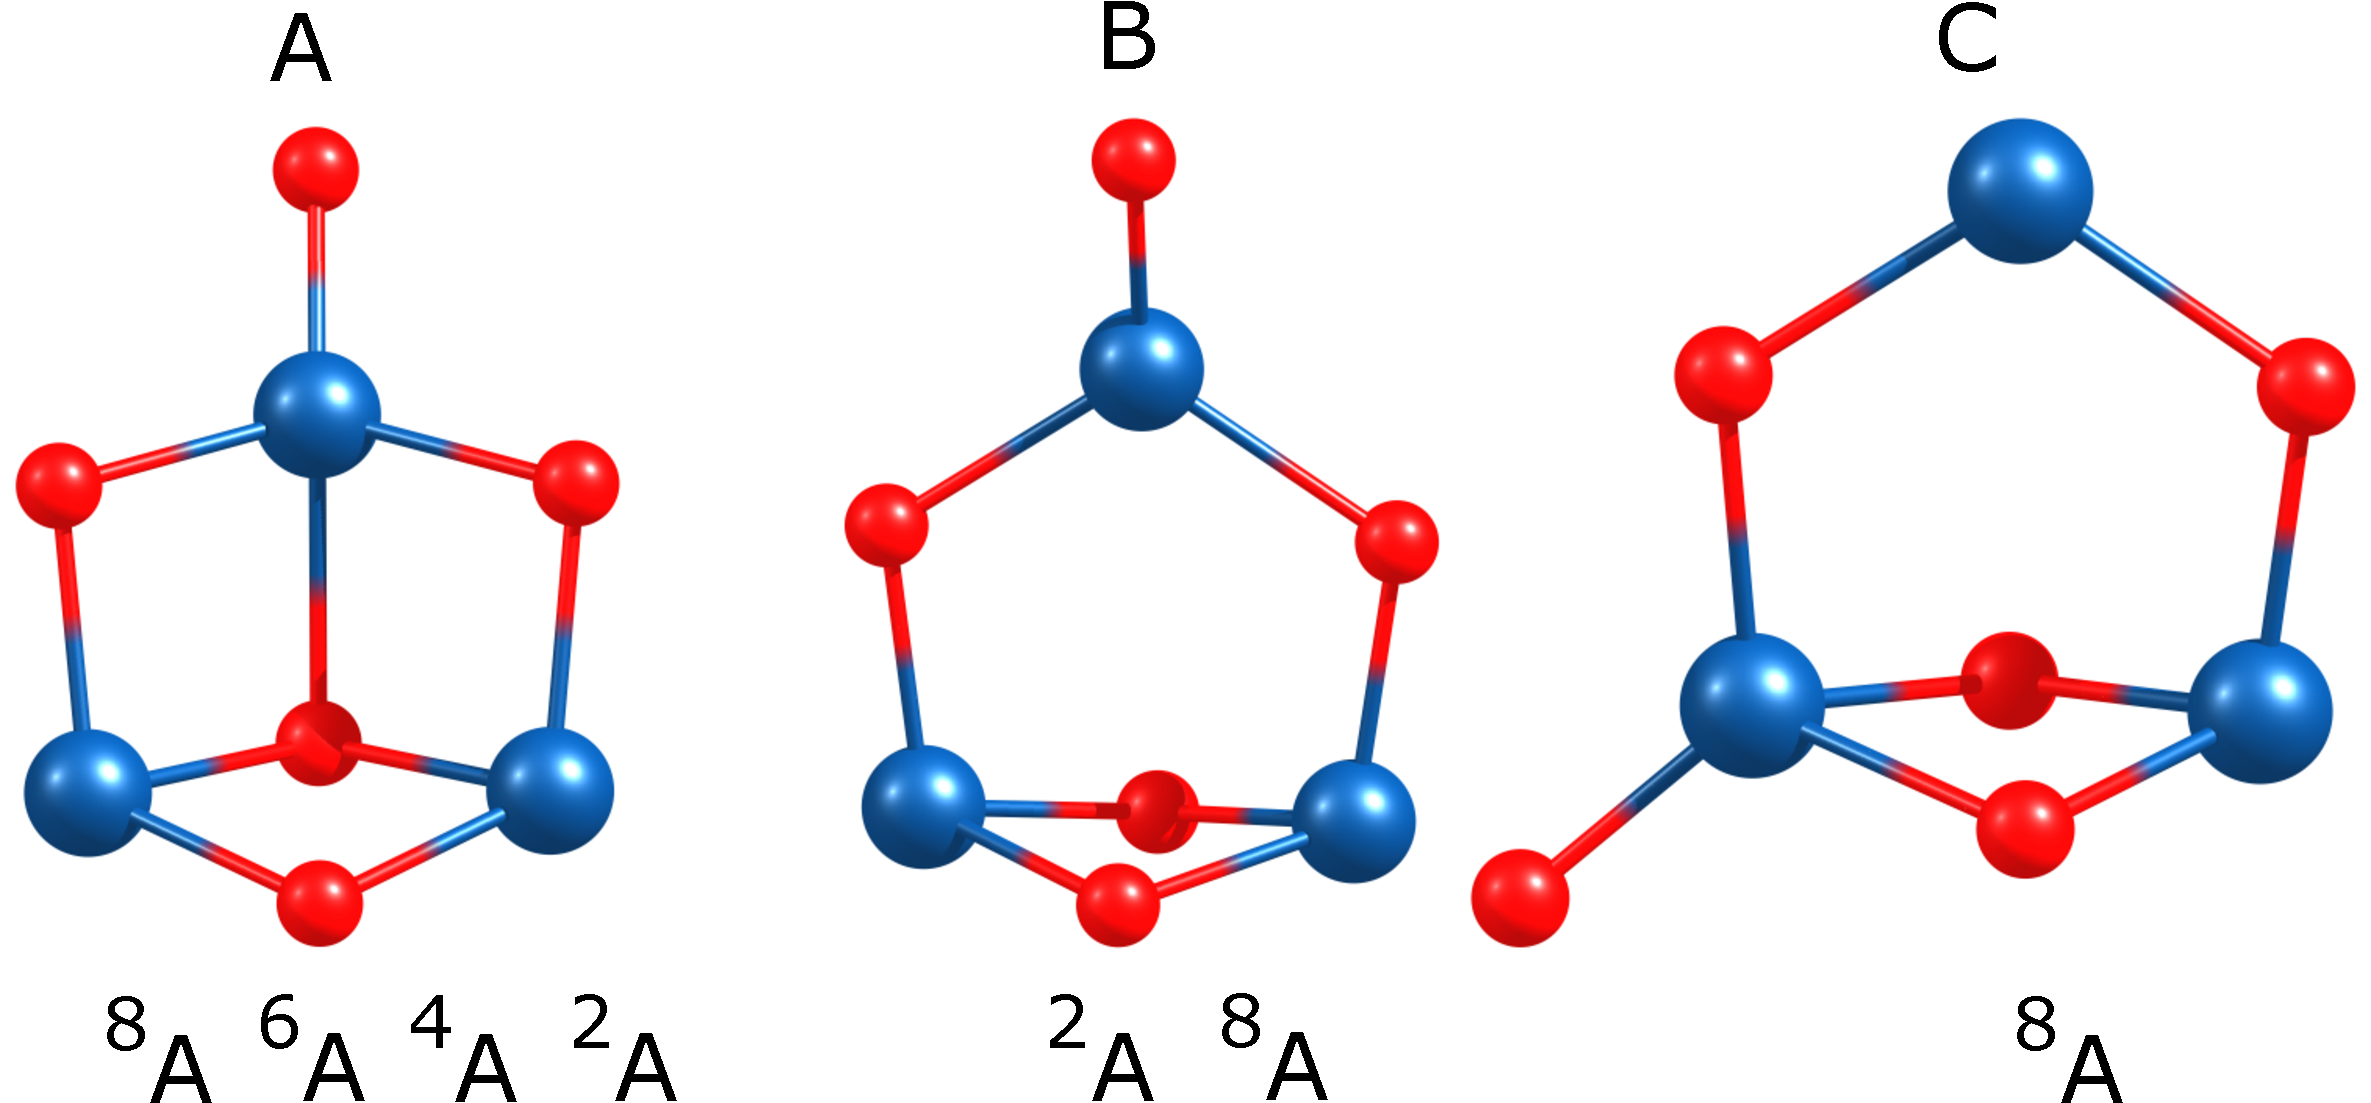
\includegraphics[width=0.52\textwidth]{Cr3O5-isomers.pdf}
	\caption{Geometrical structures of the lowest energy states of \ce{Cr3O5+}.}
	\label{a7fig:Cr3O5-isomers}
\end{figure}

\begin{figure}[]
	\centering
	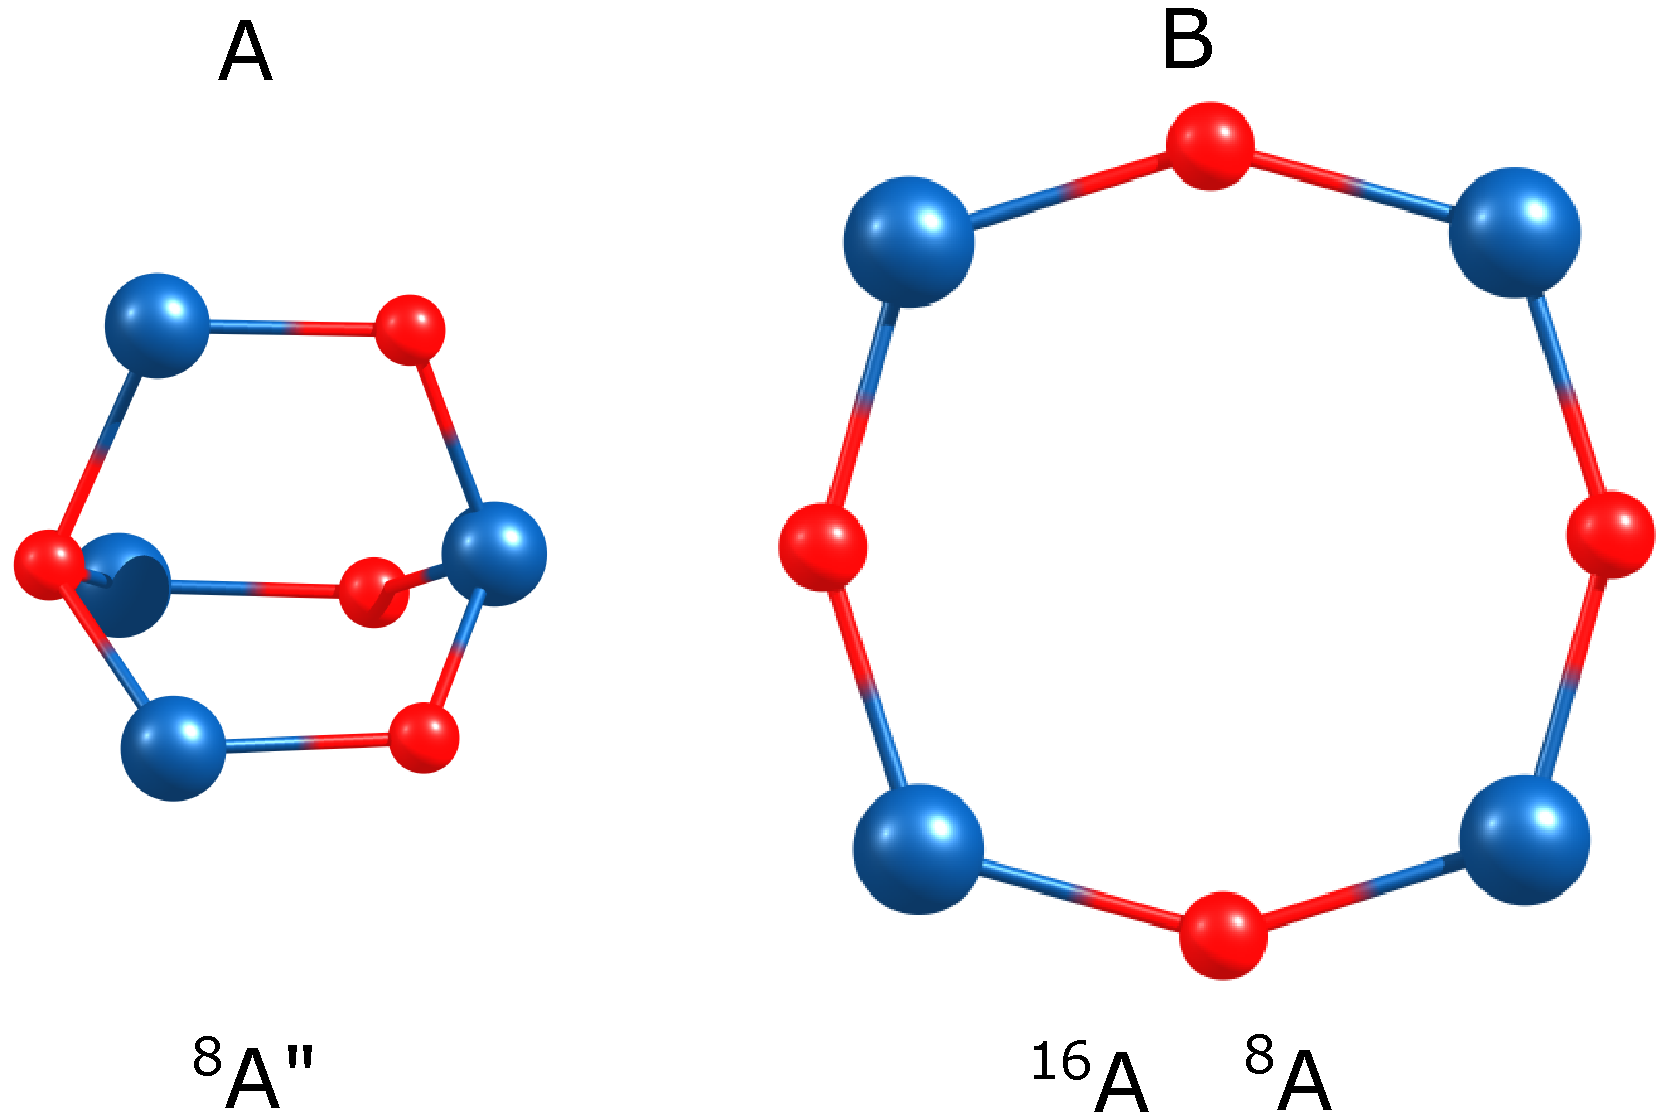
\includegraphics[width=0.45\textwidth]{Cr4O4-isomers.pdf}
	\caption{Geometrical structures of the lowest energy states of \ce{Cr4O4+}.}
	\label{a7fig:Cr4O4-isomers}
\end{figure}

\newpage

\section[Relataive energies of \ch{C\lowercase{r}3O_{\lowercase{m}}^+} (\lowercase{m} = 0 -- 5) and \ch{C\lowercase{r}4O4+}]{Relative energies of low energy isomers of \ch{Cr3O_{\lowercase{m}}^+} (\lowercase{m} = 0 -- 5) and \ch{Cr4O4+}, assessed at different \acrshort{dft} levels}

\begin{table}[h]
    \centering
    \small
	\caption{Relative energies (in eV) of the low energy isomers of \ce{Cr3+} calculated at different \acrshort{dft} levels}
	\label{a7tbl:Cr3}
	\begin{tabular}{cllllllll}
		\hline
		\multirow{2}{*}{spin state} & \multirow{2}{*}{structure} & \multicolumn{7}{c}{method}                          \\ \cline{3-9} 
		    &         & BP86 & M06L & TPSS & B3P86 & B3PW91 & B3LYP & TPSSH \\ \hline
        2   & cyclic  & 1.32 & 0.86 & 0.19 & 0.43  & 0.47   & 1.38  & 0.85  \\
        4   & cyclic  & 0.00 & 0.00 & 0.00 & 0.00  & 0.00   & 0.00  & 0.00  \\
        6   & cyclic  & 2.41 & 3.17 & 1.88 & 2.10  & -1.96  & -1.72 & 1.57  \\
        8   & cyclic  & 4.62 & 3.27 & 2.52 & 2.33  & 4.99   & 4.58  & 3.70  \\
        10  & cyclic  & 1.46 & 2.67 & 1.81 & 1.68  & 3.10   & 1.36  & 2.41  \\ \hline 
	\end{tabular}
\end{table}


\begin{table}[h]
	\centering
	\caption{Relative energies (in eV) of the low energy isomers of \ce{Cr3O+} calculated at different \acrshort{dft} levels}
	\label{a7tbl:Cr3O}
	\begin{tabular}{llrrrrrrr}
		\hline
		\multirow{2}{*}{state} & \multirow{2}{*}{sym.}  & \multicolumn{7}{c}{method}                                  \\ \cline{3-9} 
						 &            & BP86   & M06L  & TPSS  & B3P86   & B3LYP  & B3PW91   & TPSSh       	\\ \hline
        $^6$A$'$         & C$_s$      & 0.00   & 0.00  & 0.00  & 0.00    & 0.00   & 0.00     & 0.00  		\\
        $^{16}$A$'$      & D$_{3h}$   & 0.22   & 0.79  & 0.33  & 0.15    & 0.16   & 0.33     & 0.10  		\\
        $^4$A$_1$        & C$_{2v}$   & 0.96   & 0.73  & 0.89  & 1.10    & 0.85   & 0.85     & 0.94  		\\
        $^{14}$A$'$      & C$_s$      & 1.01   & 0.63  & 0.81  & 1.04    & 0.80   & 0.79     & 0.96  		\\
        $^{14}$A$_1$     & C$_{2v}$   & 1.16   & 1.00  & 1.06  & 1.44    & 1.30   & 1.06     & 1.14  		\\ \hline
	\end{tabular}
\end{table}


\begin{table}[h]
    \centering
    \small
	\label{a7tbl:Cr3O2}
	\caption{Relative energies (in eV) of the low energy isomers of \ce{Cr3O2+} calculated at different \acrshort{dft} levels}
	\begin{tabular}{lllrrrrrrr}
		\hline
		\multirow{2}{*}{state} & \multirow{2}{*}{isomer} & \multirow{2}{*}{sym.} & \multicolumn{7}{c}{method}   \\ \cline{4-10} 
							   &      &           & BP86  & M06L & TPSS   & B3P86 & B3LYP  & B3PW91 & TPSSH \\ \hline
        $^6 $A                 & A    & C$_1$     & 0.00  & 0.00 & 0.00   & 0.00  & 0.00   & 0.00   & 0.00  \\
        $^{14}$A$^\prime$      & B    & C$_s$     & 0.16  & 0.45 & 0.11   & 0.07  & 0.08   & 0.06   & 0.03  \\
        $^{14}$A$_2$           & C    & C$_{2v}$  &       & 0.06 &        & 0.17  & 0.14   & 0.11   &       \\
        $^{14}$A$_2$           & D    & C$_{2v}$  & -0.25 & 0.25 & -0.15  & 0.35  & 0.31   & 0.28   & 0.07  \\ \hline
	\end{tabular}
\end{table}


\begin{table}[h]
    \centering
    \small
	\caption{Relative energies (in eV) of the low energy isomers of \ce{Cr3O3+} calculated at different \acrshort{dft} levels}
	\label{a7tbl:Cr3O3}
	\begin{tabular}{lllrrrrrrr}
		\hline
		\multirow{2}{*}{state} & \multirow{2}{*}{isomer} & \multirow{2}{*}{sym.} & \multicolumn{7}{c}{method}                           \\ \cline{4-10} 
							&      &       & BP86  & M06L & TPSS  & B3P86 & B3LYP   & B3PW91  & TPSSH \\ \hline
     $^{12}$A$'$    		& A    & C$_s$ & 0.00  & 0.00 & 0.00  & 0.00  & 0.00    & 0.00    & 0.00  \\
      $^{12}$A          	& B    & C$_1$ & 0.40  & -0.05& 0.14  & -0.02 & 0.17    & 0.10    & 0.06  \\
      $^{10}$A          	& B    & C$_1$ & 0.95  & 1.10 & 1.04  & 1.17  & 1.28    & 1.19    & 1.05  \\
      $^{10}$A          	& C    & C$_1$ & 0.95  & 0.94 & 1.04  & 1.01  & 1.09    & 1.19    & 0.77  \\
      $ ^8  $A          	& D    & C$_1$ & 1.07  & 0.94 & 0.46  & 0.87  & 0.68    & 1.06    & 0.87  \\ \hline
	\end{tabular}
\end{table}


\begin{table}[h]
    \centering
    \small
	\caption{Relative energies (in eV) of the low energy isomers of \ce{Cr3O4+} calculated at different \acrshort{dft} levels}
	\label{a7tbl:Cr3O4}
	\begin{tabular}{clllllllll}
		\hline
		\multirow{2}{*}{state} & \multirow{2}{*}{isomer} & \multirow{2}{*}{sym.} & \multicolumn{7}{c}{method}                          \\ \cline{4-10} 
				  &      &         & BP86 & M06L & TPSS  & B3P86  & B3PW91  & B3LYP & TPSSH \\ \hline 
        $^{10}$A  & A    & C$_1$   & 0.00 & 0.00 & 0.00  & 0.00   & 0.00    & 0.00  & 0.00  \\
        $^4$A     &      &         & 0.71 & 0.11 & 0.02  & 2.58   & 2.65    & 2.56  & 1.40  \\
        $^{10}$A  & B    & C$_1$   & 0.12 & 0.59 & 0.56  & 0.74   & 0.58    & 0.51  & 0.88  \\
        $^6$A     &      &         & 0.03 & 2.33 & 0.50  & 1.99   & 1.92    & 1.35  & 1.83  \\
        $^{10}$A  & C    & C$_1$   & 0.05 & 0.49 & 0.30  & 0.65   & 0.57    & 0.57  & 0.60  \\
        $^{10}$A  & D    & C$_1$   & 0.52 & 0.73 & 0.80  & 0.72   & 0.65    & 0.65  & 0.89  \\
        $^6$A     &      &         & 0.44 & 2.40 & 0.74  & 2.84   & 2.88    & 2.12  & 2.03  \\ \hline
	\end{tabular}                               
\end{table}


\begin{table}[h]
    \centering
    \small
	\caption{Relative energies (in eV) of the low energy isomers of \ce{Cr3O5+} calculated at different \acrshort{dft} levels}
	\label{a7tbl:Cr3O5}
	\begin{tabular}{clllllllll}
		\hline
		\multirow{2}{*}{state} & \multirow{2}{*}{isomer} & \multirow{2}{*}{sym.} & \multicolumn{7}{c}{method}                          \\ \cline{4-10} 
			   &      &         & BP86 & M06L  & TPSS  & B3P86  & B3PW91 & B3LYP & TPSSH \\ \hline 
        $^8$A  & A    & C$_1$   & 0.00 & 0.00  & 0.00  & 0.00   & 0.00   & 0.00  & 0.00  \\
        $^4$A  &      &         & 0.47 & 0.61  & 0.13  & 0.95   & 0.94   & 0.88  & 0.18  \\
        $^6$A  &      &         & 0.59 & 1.03  & 0.09  & 0.86   & 0.91   & 0.86  & 0.16  \\
        $^2$A  &      &         & 0.68 & 0.13  & 0.20  & 1.79   & 0.99   & 1.76  & 0.90  \\
        $^2$A  & B    & C$_1$   & 0.22 & 0.55  & -0.06 & 1.02   & 1.00   & 0.55  & 0.14  \\
        $^8$A  &      &         & 0.37 & 0.61  & 0.11  & 0.69   & 0.64   & 0.56  & 0.21  \\
        $^8$A  & C    & C$_1$   & 0.11 & 0.21  & -0.15 & 0.63   & 0.55   & 0.54  & 0.04  \\ \hline
	\end{tabular}                               
\end{table}

\begin{table}[h]
    \centering
    \small
	\caption[Relative energies of of \ce{Cr4O4+}]{Relative energies (in eV) of the low energy isomers of \ce{Cr4O4+} calculated at different \acrshort{dft} levels}
	\label{a7tbl:Cr4O4}
	\begin{tabular}{lllrrrrrrr}
		\hline
		\multirow{2}{*}{state} & \multirow{2}{*}{isomer} & \multirow{2}{*}{sym.} & \multicolumn{7}{c}{method}\\ \cline{4-10} 
					   &      &        & BP86 & M06L & TPSS & B3P86 & B3LYP  & B3PW91  & TPSSH 	   \\ \hline
		$^8$A$''$      & A    & C$_s $ & 0.00 & 0.00 & 0.00 & 0.00  &  0.00  & 0.00    & 0.00  		\\
		$^{16}$A       & B    & C$_1 $ & 0.13 & 0.34 & 0.19 & 0.18  & -0.09  & 0.09    &       		\\
		$^8$A          & B    & C$_1 $ & 0.27 & 0.59 & 0.45 & 0.16  &  0.17  &         &       		\\ \hline
	\end{tabular}
\end{table}


\clearpage
\section[Simulated versus Experimental Spectra]{Comparison of the experimental \acrshort{irpd} spectra of \ce{Cr2O2+}, \ce{Cr3O+}, \ce{Cr3O2+}, \ce{Cr3O3+}, and \ce{Cr4O4+} with calculated \acrshort{ir} spectra at different \acrshort{dft} levels}

Figure \ref{a7fig:Cr2O2-IR} shows the calculated vibrational spectra of the lowest energy $^8$B$_{1g}$ and $^8$B$_{1u}$ states of the $D_{2h}$ isomer of \ce{Cr2O2+}, as obtained using different \acrshort{dft} functionals. As can be seen the harmonic \acrshort{ir} spectra at the different \acrshort{dft} levels are consistent with one another. The only difference is the frequency of the low energy mode. In this sense the MO6L and BP86 levels seem less accurate, as the predicted $400 - 450$ cm$^{-1}$ mode is not observed experimentally. The harmonic \acrshort{ir} spectrum of the excited state \ce{^8B_{1u}} could not be accessed at the TPSS level, for that reason the results obtained at the B3P86 level are used in Figure 1b of the manuscript. 

Calculated vibrational spectra of the lowest energy isomers of the other clusters (\ce{Cr3O+}, \ce{Cr3O2+}, \ce{Cr3O3+}, and \ce{Cr4O4+}) also show a good consistency with one another. Main differences are in the exact position of the observed vibrational modes, which is typically addressed by scaling factors. The TPSS functional, which was opted for in the main text, does not require systematic scaling of the vibrational modes. 

\begin{figure}[]
	\centering
	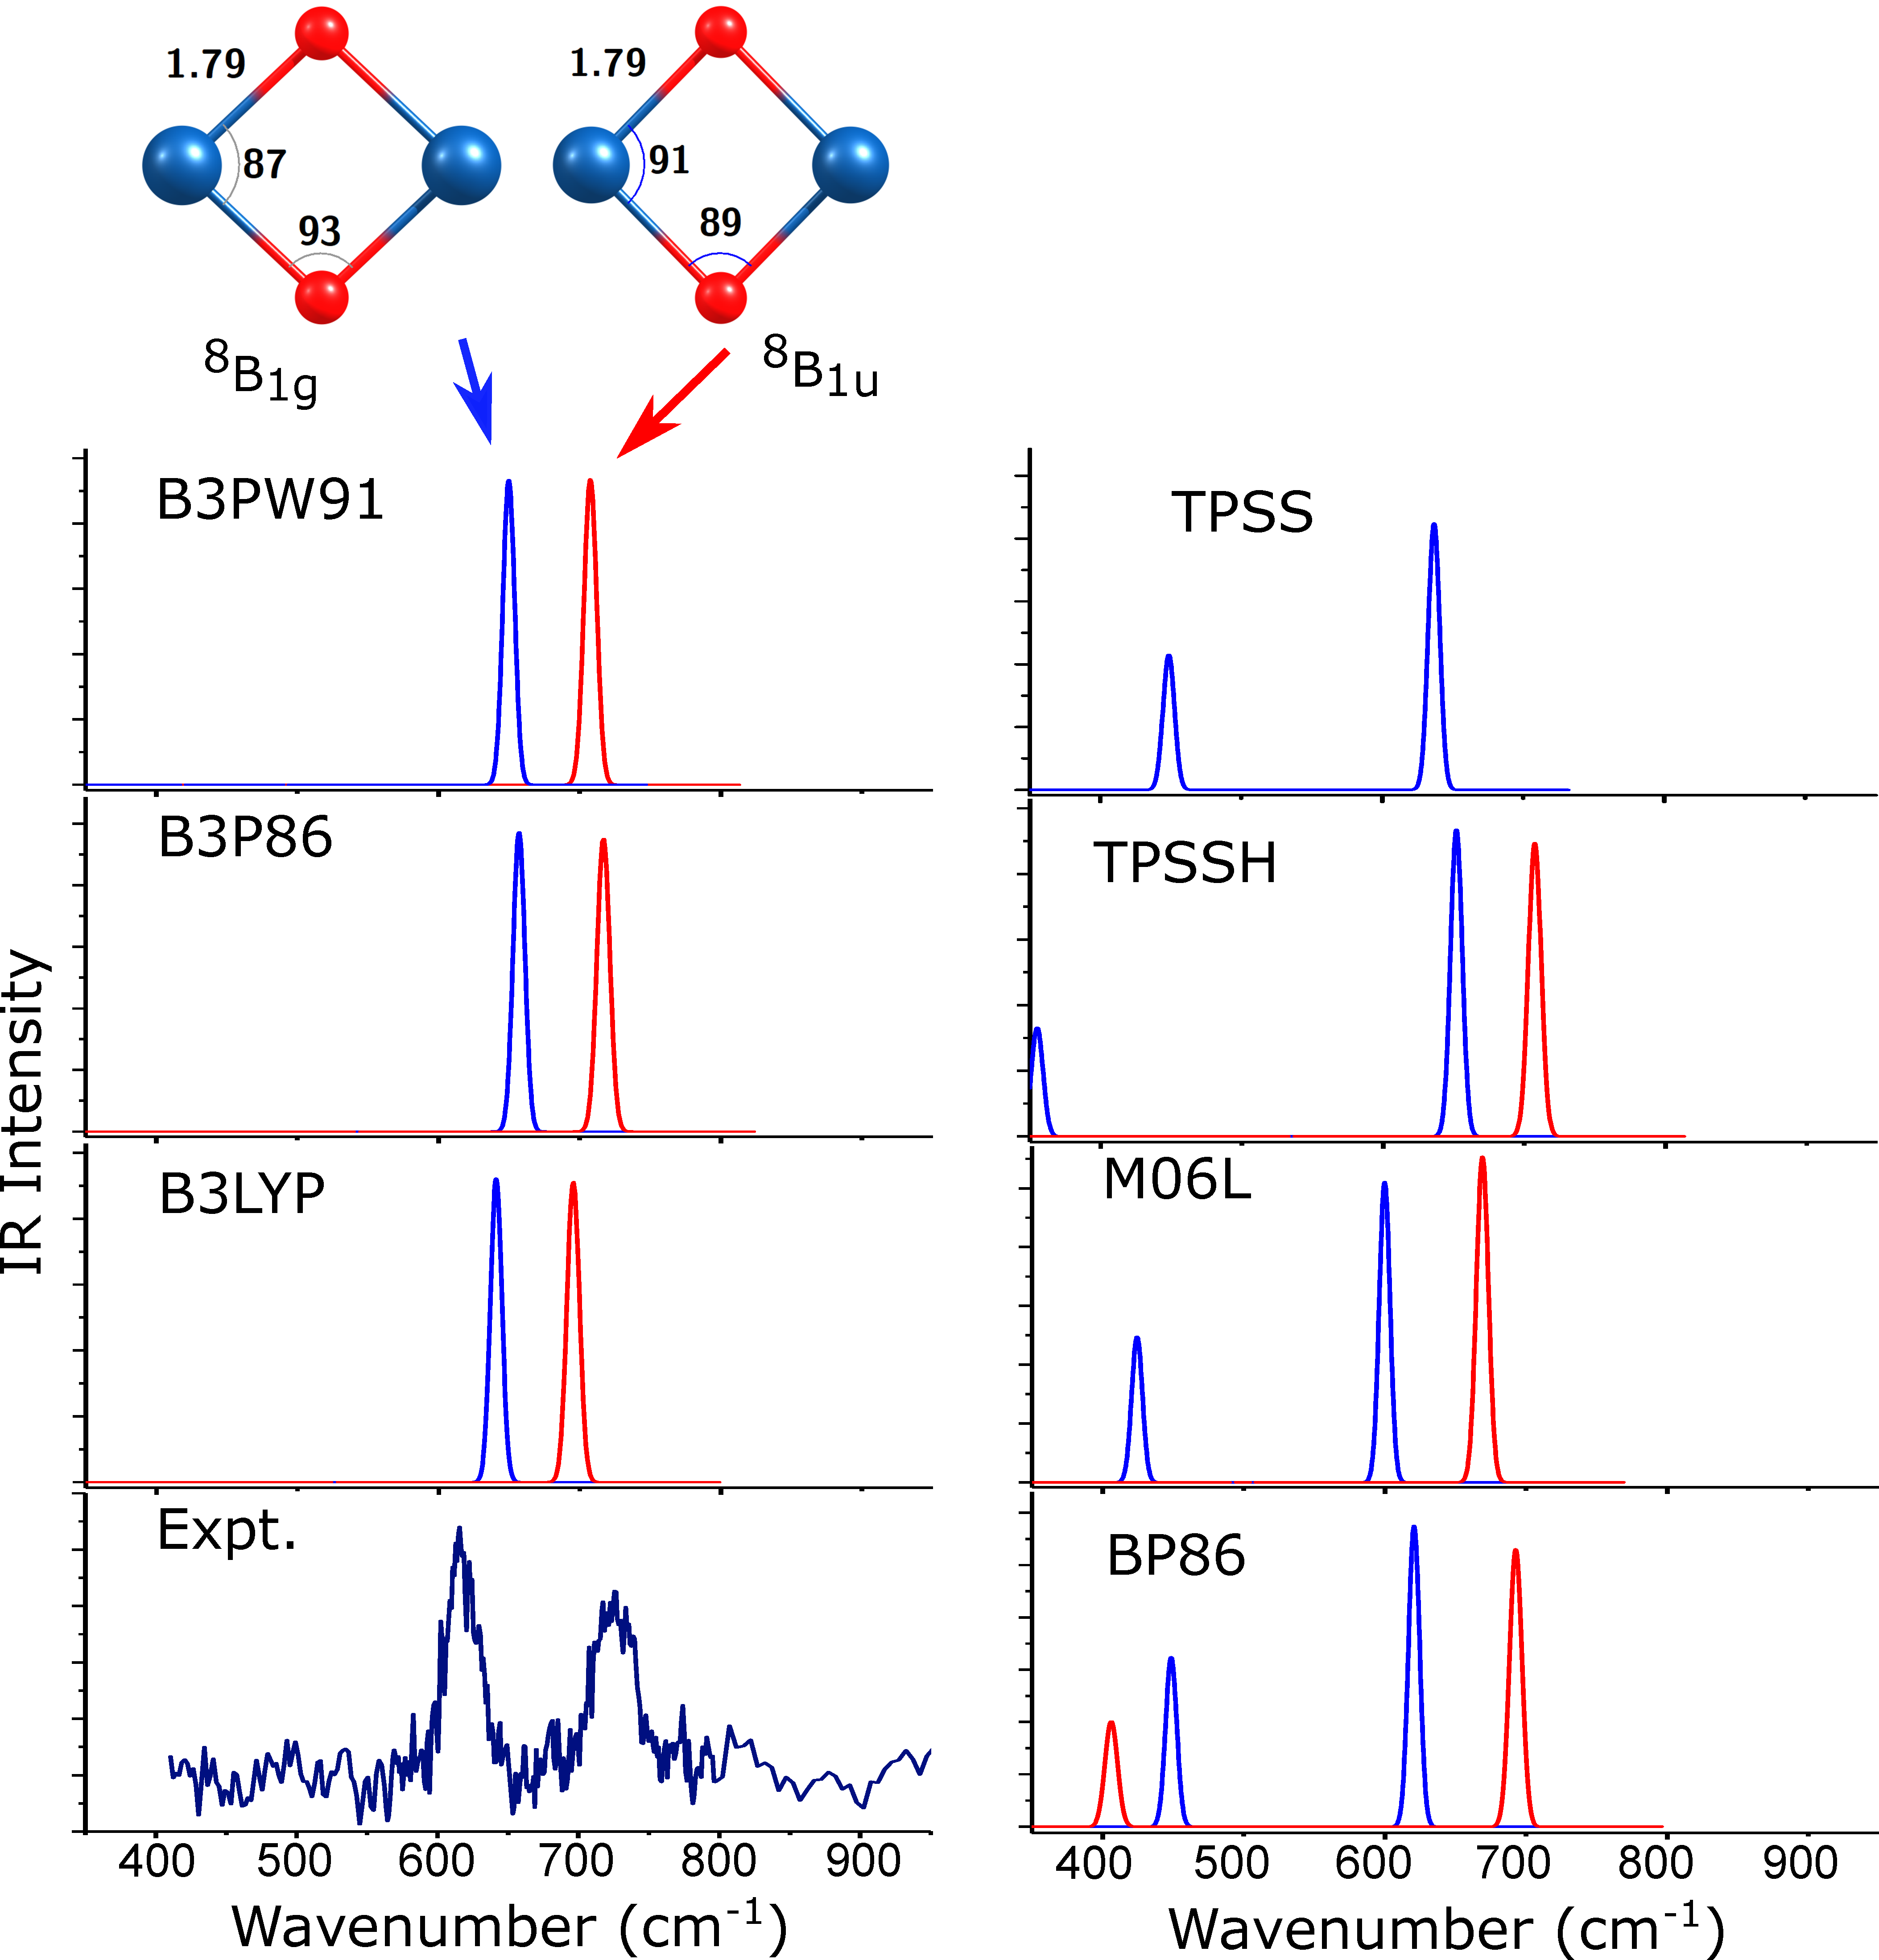
\includegraphics[width=0.8\textwidth]{Cr2O2-IR.pdf}
	\caption{The experimental \acrshort{irpd}  spectrum of \ce{Cr2O2+} and simulated infrared spectra for the two lowest electronic states using different \acrshort{dft} functionals. The population rates of these two states were arbitrarily set to 1:1. Simulated spectra of the $^8$B$_{1g}$ ground state and the $^8$B$_{1u}$ first excited state are given blue and red, respectively. Chromium and oxygen atoms are represented by blue and red balls, respectively. The \acrshort{irpd}  spectra were measured by monitoring predissociation of \ce{Cr2O2+}$\boldsymbol{\cdot}$Ne.}
	\label{a7fig:Cr2O2-IR}
\end{figure}

\begin{figure}[]
	\centering
	\includegraphics[width=0.8\textwidth]{Cr3O-IR.pdf}
	\caption{The experimental \acrshort{irpd}  spectrum of \ce{Cr3O+} and simulated infrared spectra for the two lowest electronic states using different \acrshort{dft} functionals ($^6$A$'$ ground state and $^{16}$A$'$ first excited state). Chromium and oxygen atoms are represented by blue and red balls, respectively.}
	\label{a7fig:Cr3O-IR}
\end{figure}

\begin{figure}[]
	\centering
	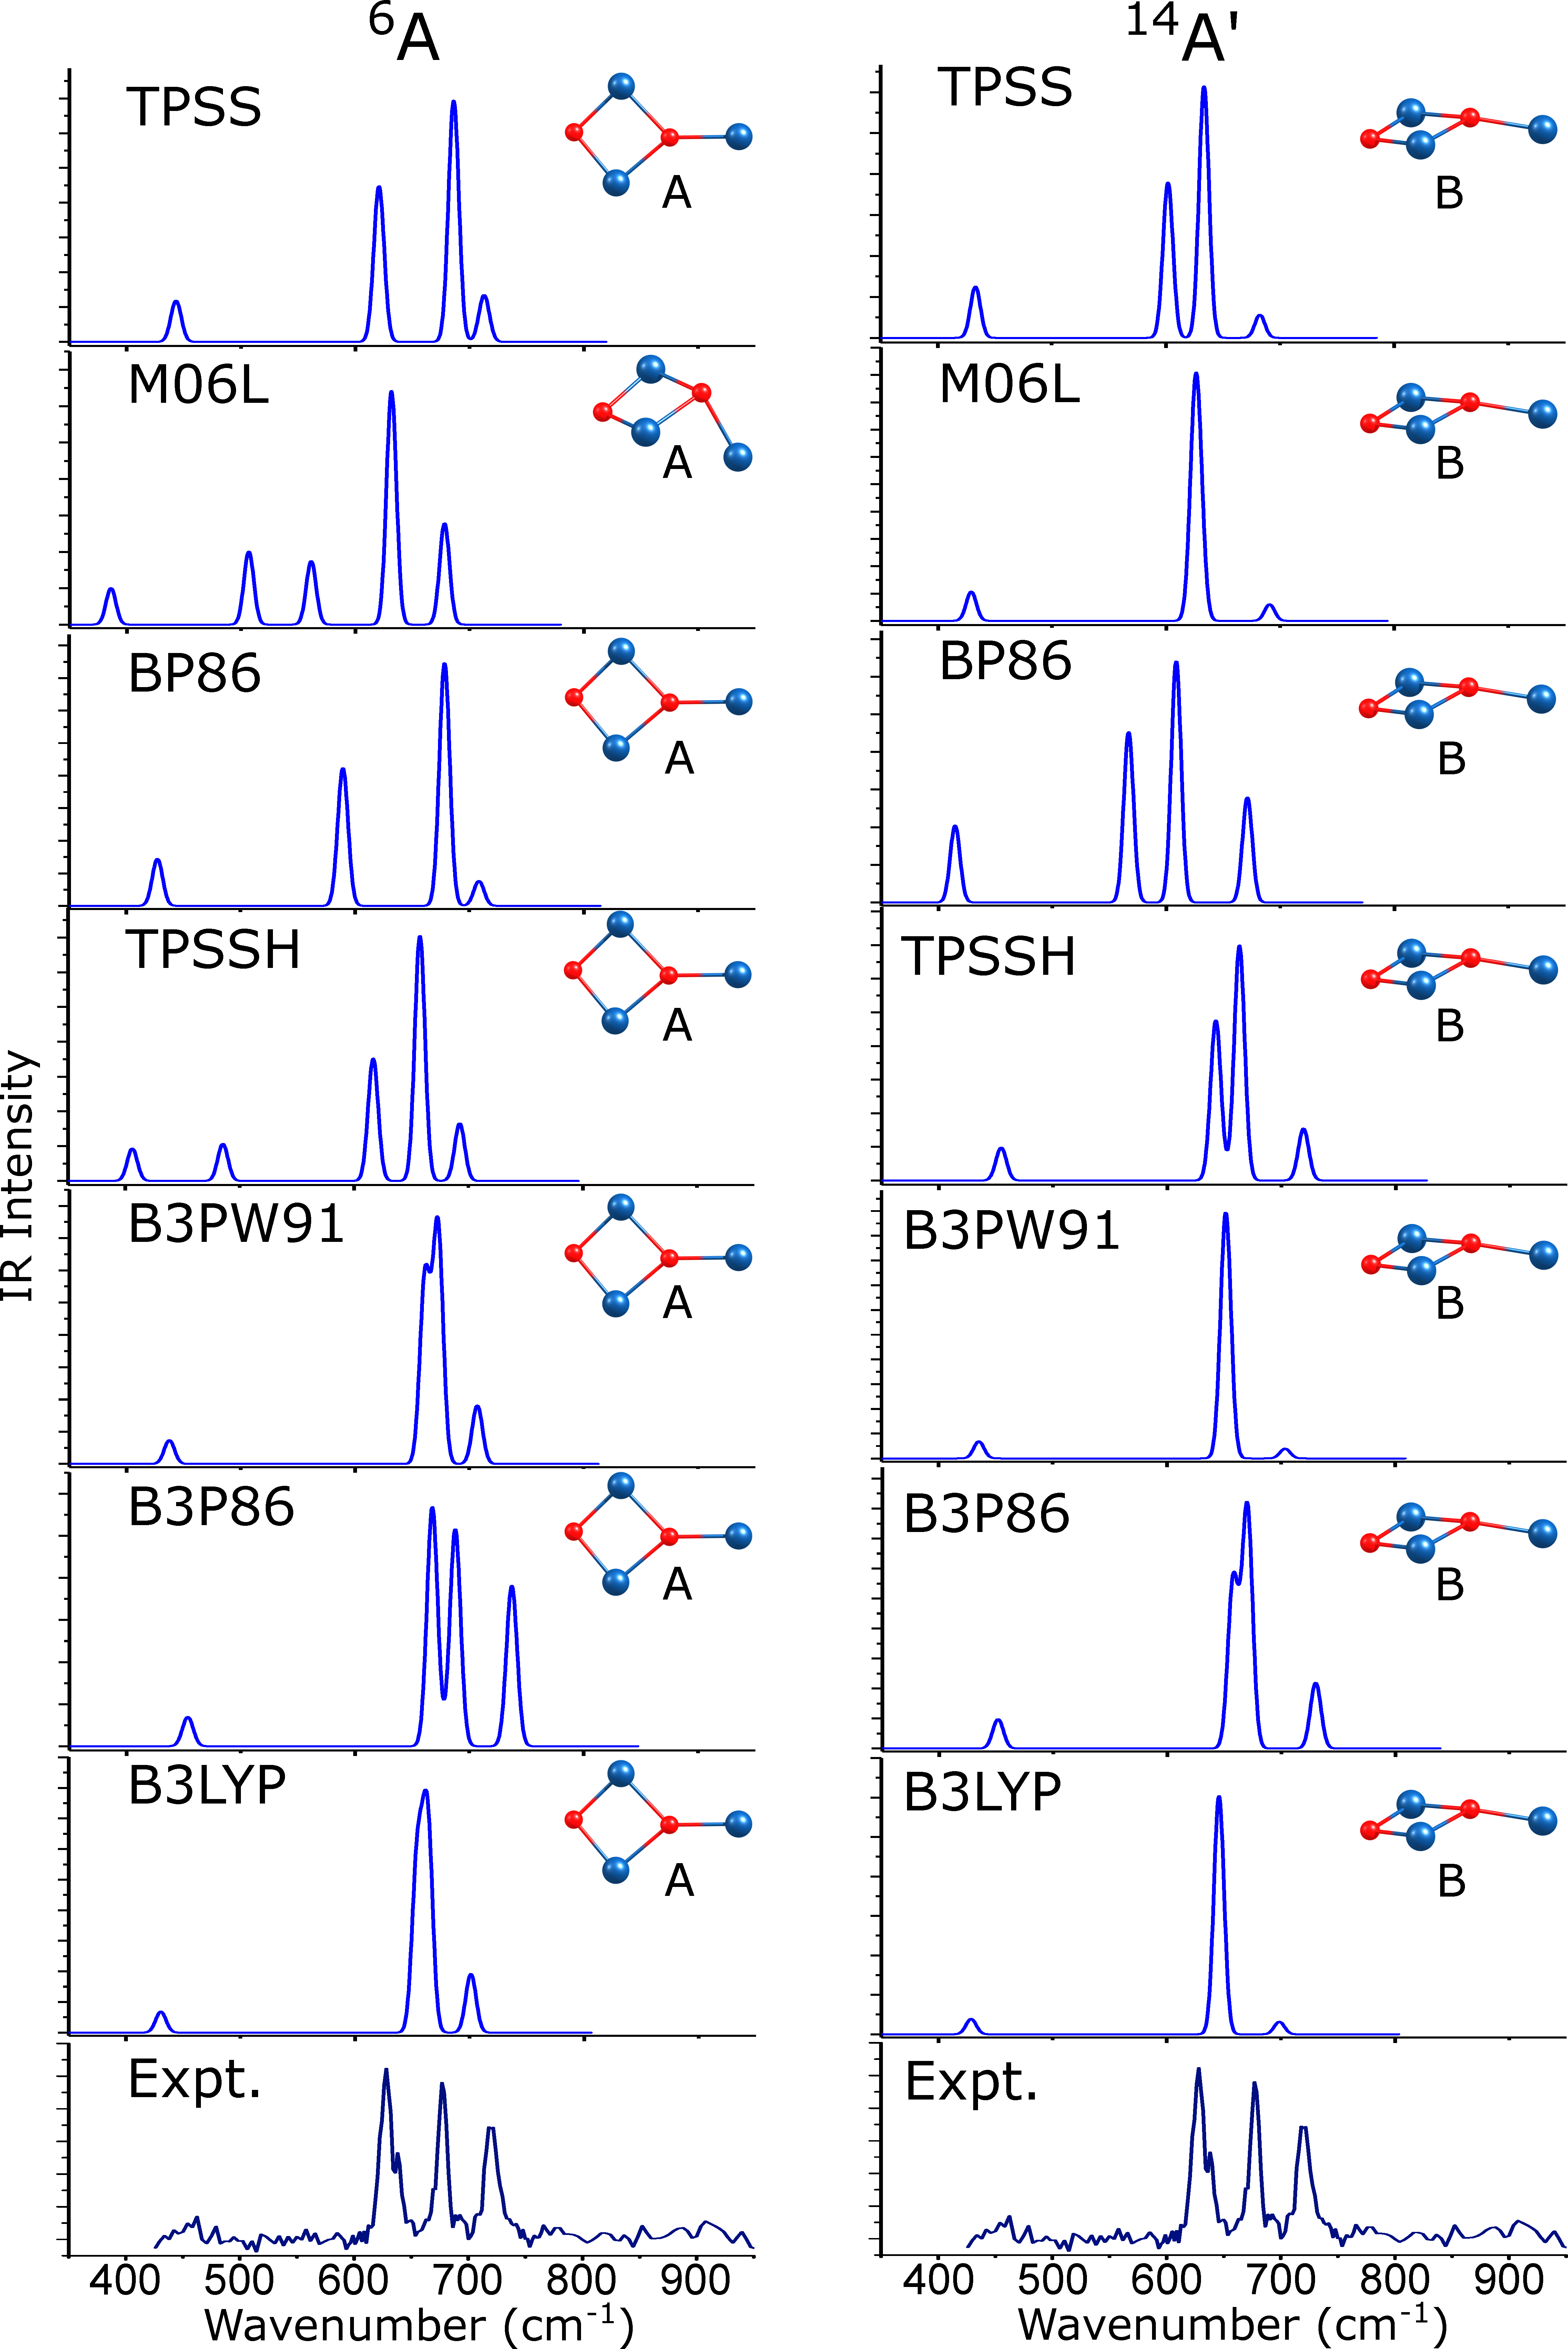
\includegraphics[width=0.8\textwidth]{Cr3O2-IR.pdf}
	\caption{The experimental \acrshort{irpd}  spectrum of \ce{Cr3O2+} and simulated infrared spectra for the two lowest electronic states using different \acrshort{dft} functionals ($^6$A ground state and $^{14}$A$'$ first excited state). Chromium and oxygen atoms are represented by blue and red balls, respectively.}
	\label{a7fig:Cr3O2-IR}
\end{figure}

\begin{figure}[]
	\centering
	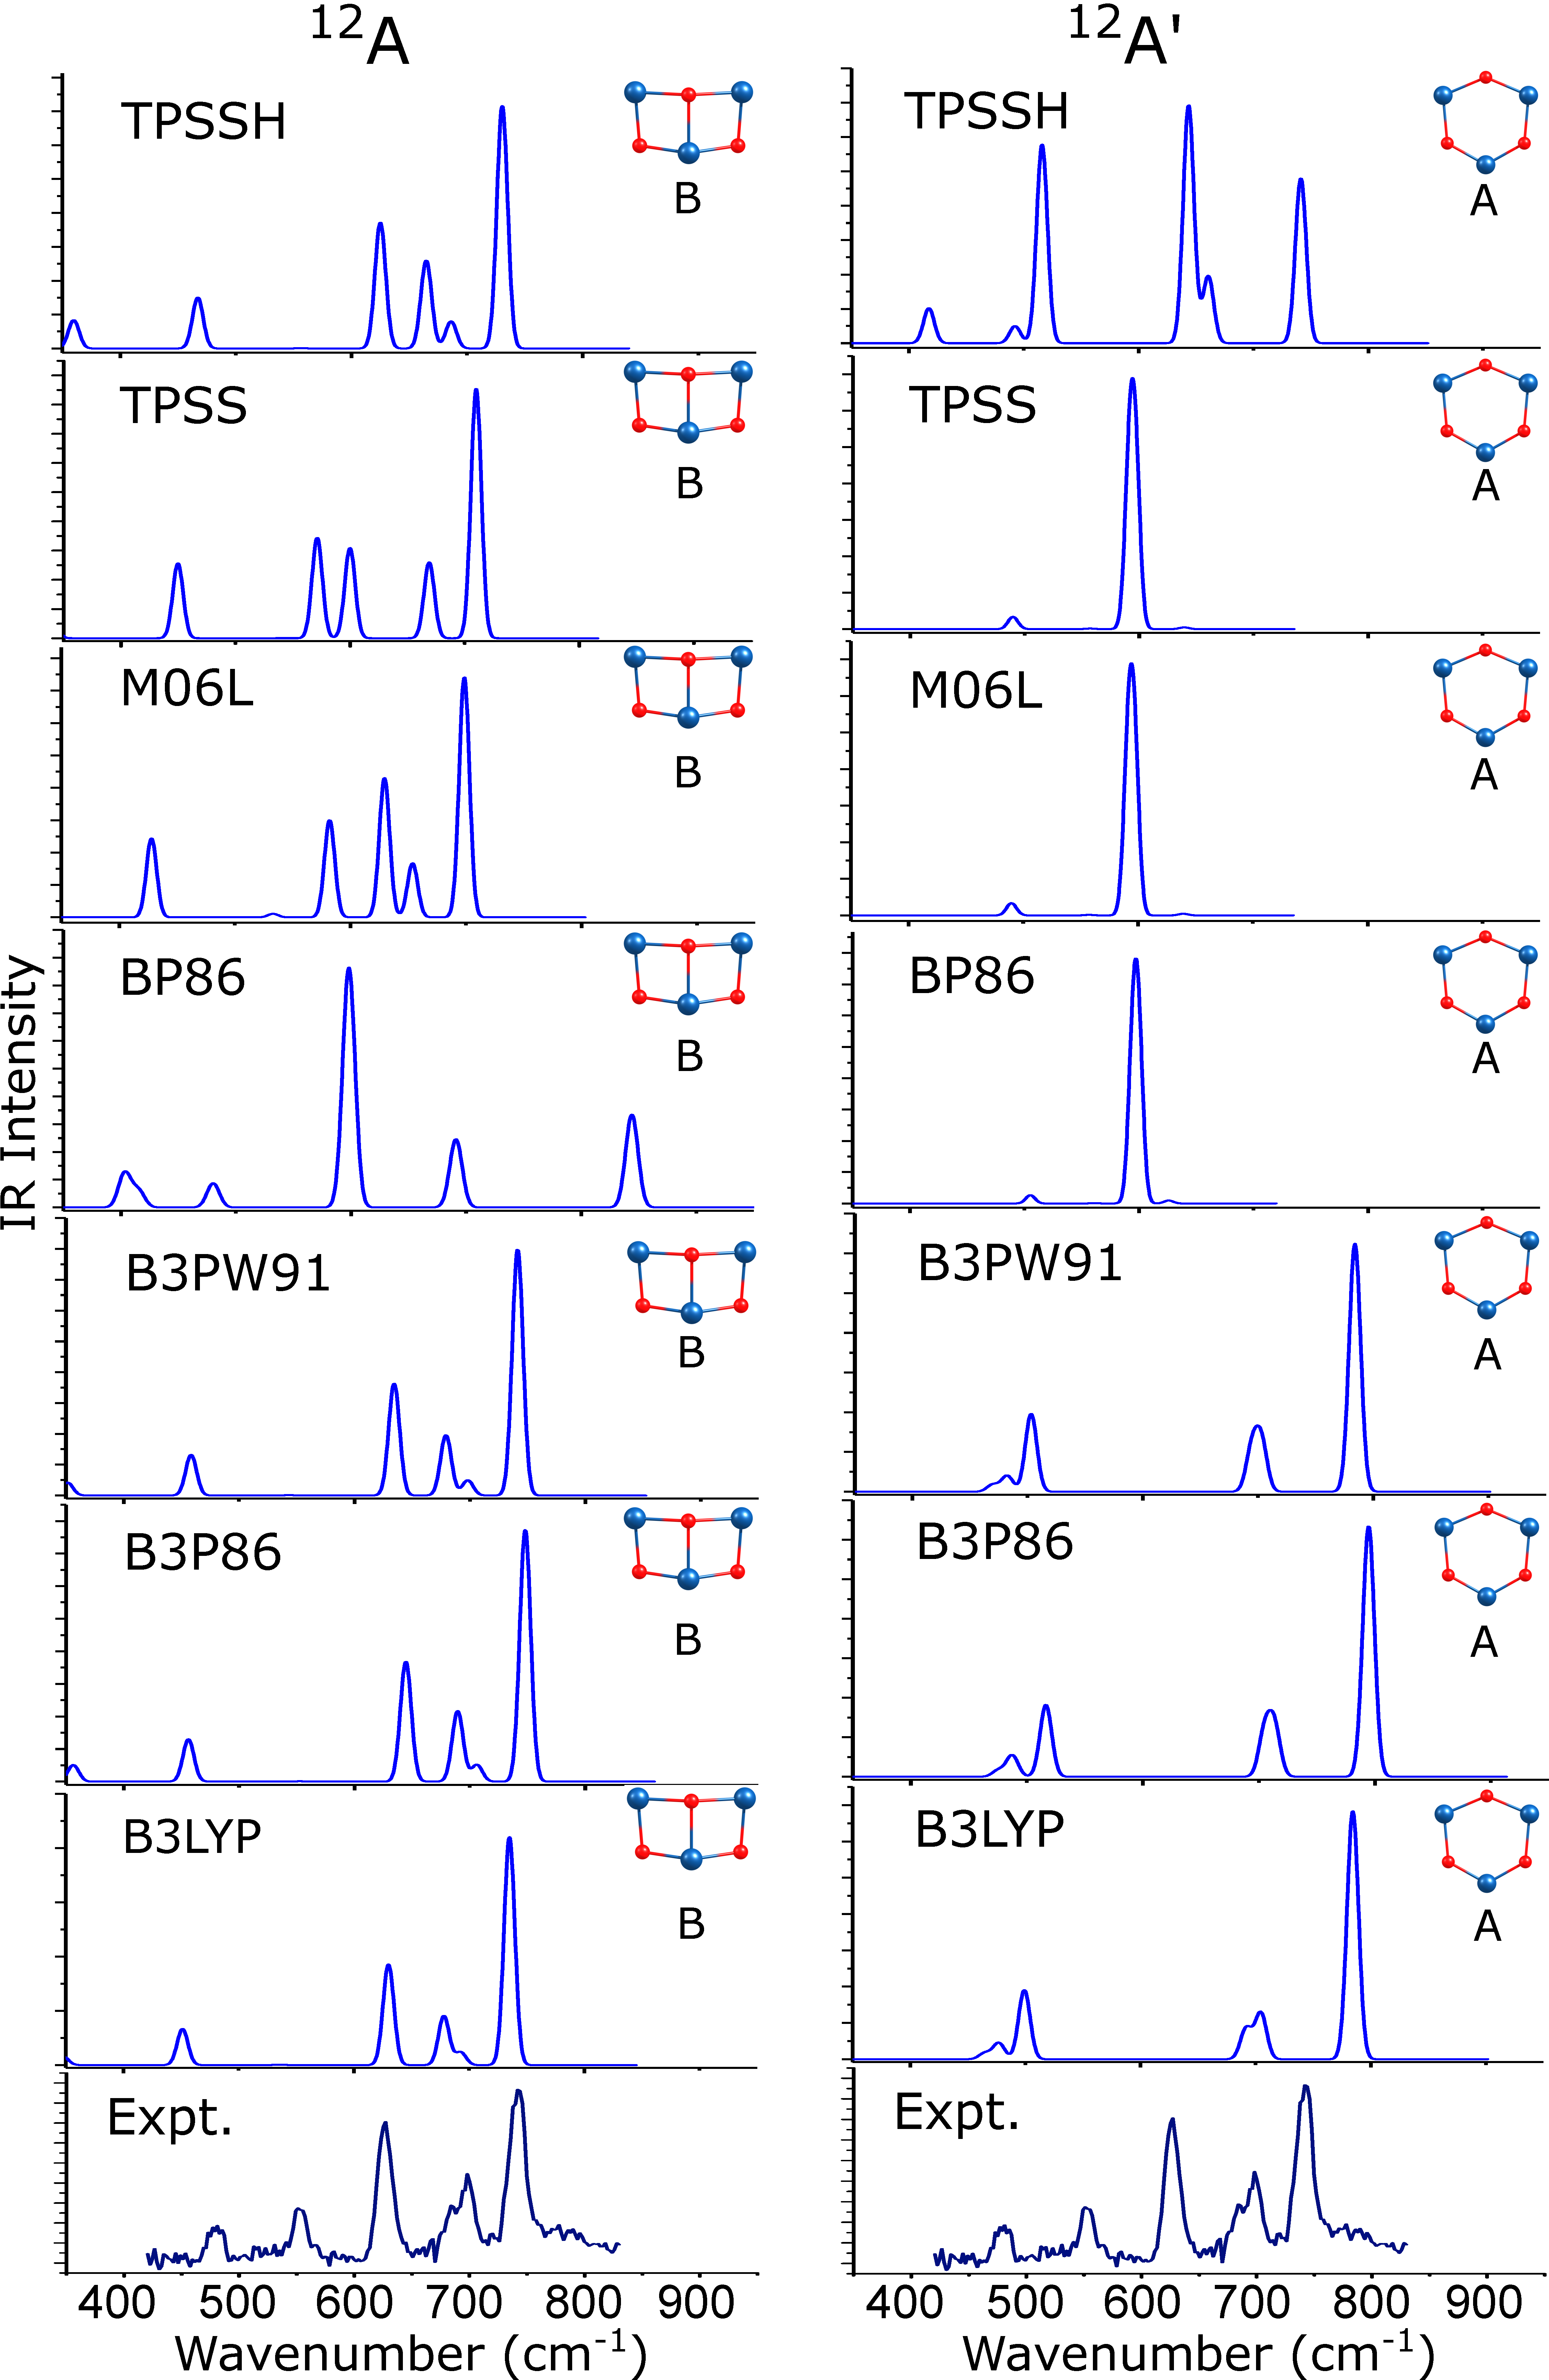
\includegraphics[width=0.8\textwidth]{Cr3O3-IR.pdf}
	\caption{The experimental \acrshort{irpd}  spectrum of \ce{Cr3O3+} and simulated infrared spectra for the two lowest electronic states using different \acrshort{dft} functionals ($^{12}$A ground state and  $^{12}$A$'$ first excited state). Chromium and oxygen atoms are represented by blue and red balls, respectively.}
	\label{a7fig:Cr3O3-IR}
\end{figure}

\begin{figure}[]
	\centering
	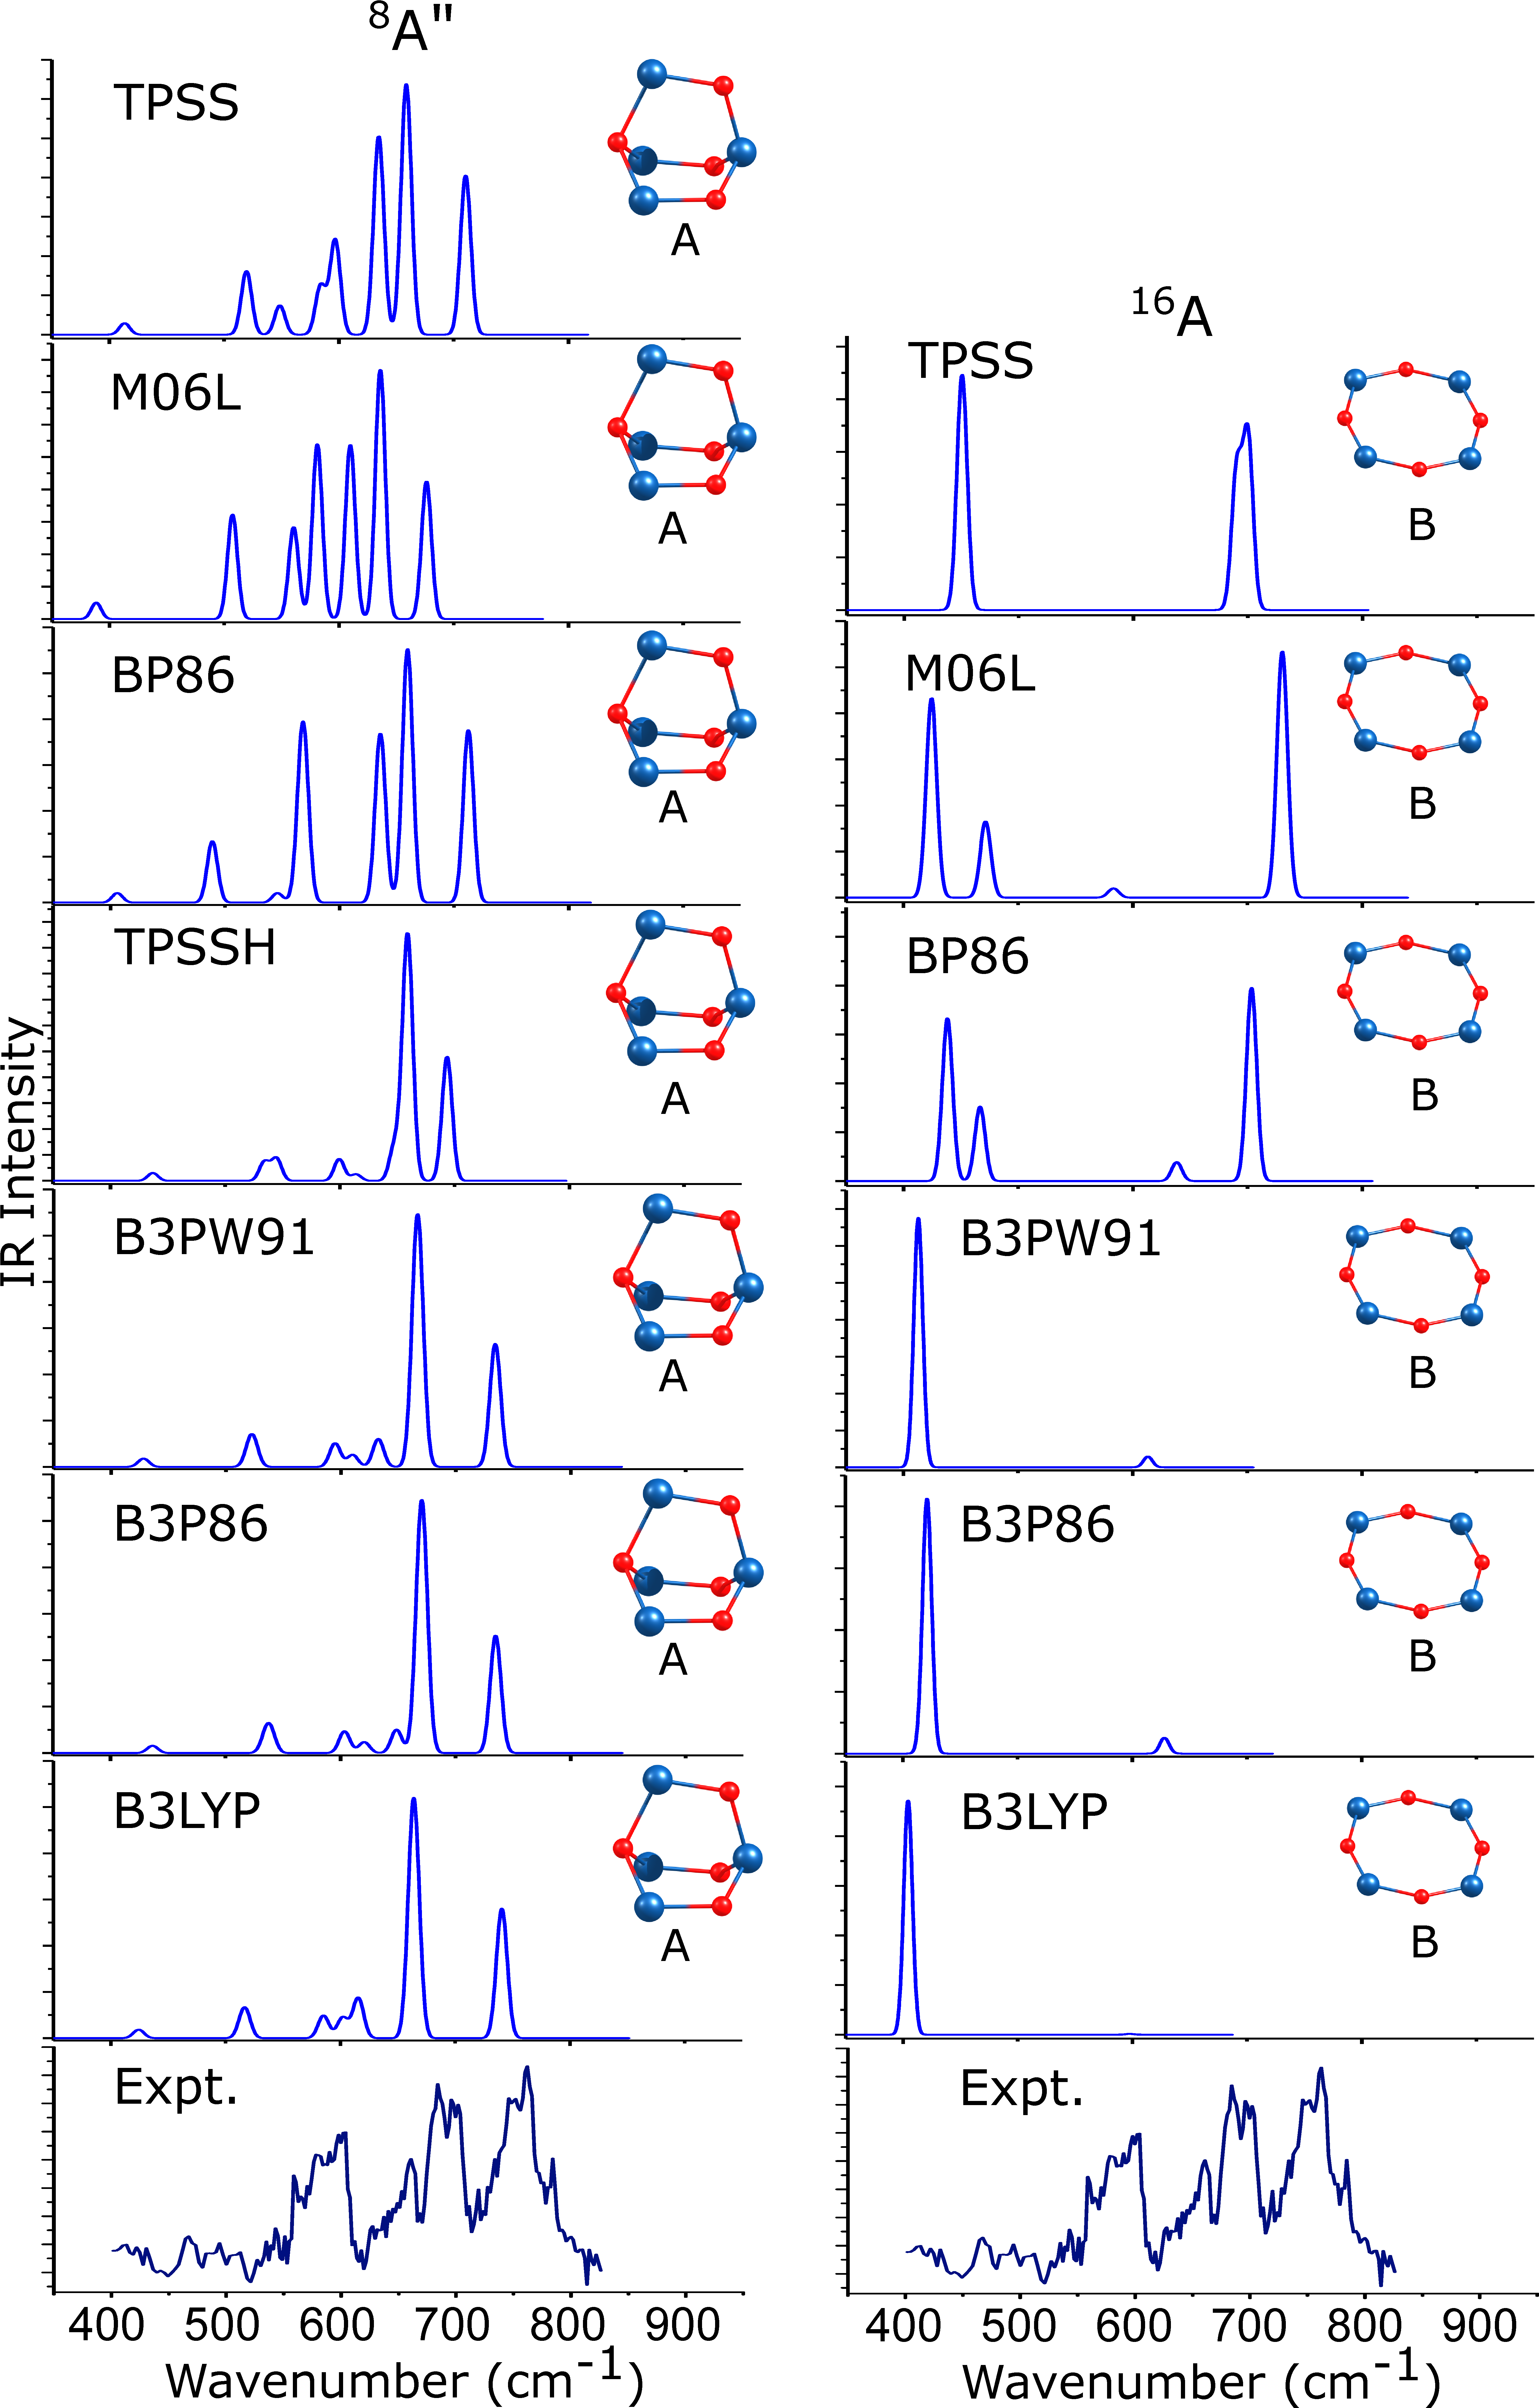
\includegraphics[width=0.8\textwidth]{Cr4O4-IR.pdf}
	\caption{Simulated and experimental infrared spectra of the ground state and its closest low-lying state.}
	\label{a7fig:Cr4O4-IR}
\end{figure}

\FloatBarrier
\newpage


\section{Possible two-center bonding-type formation from AdNDP analysis}

\begin{figure}[ht!]
	\centering
	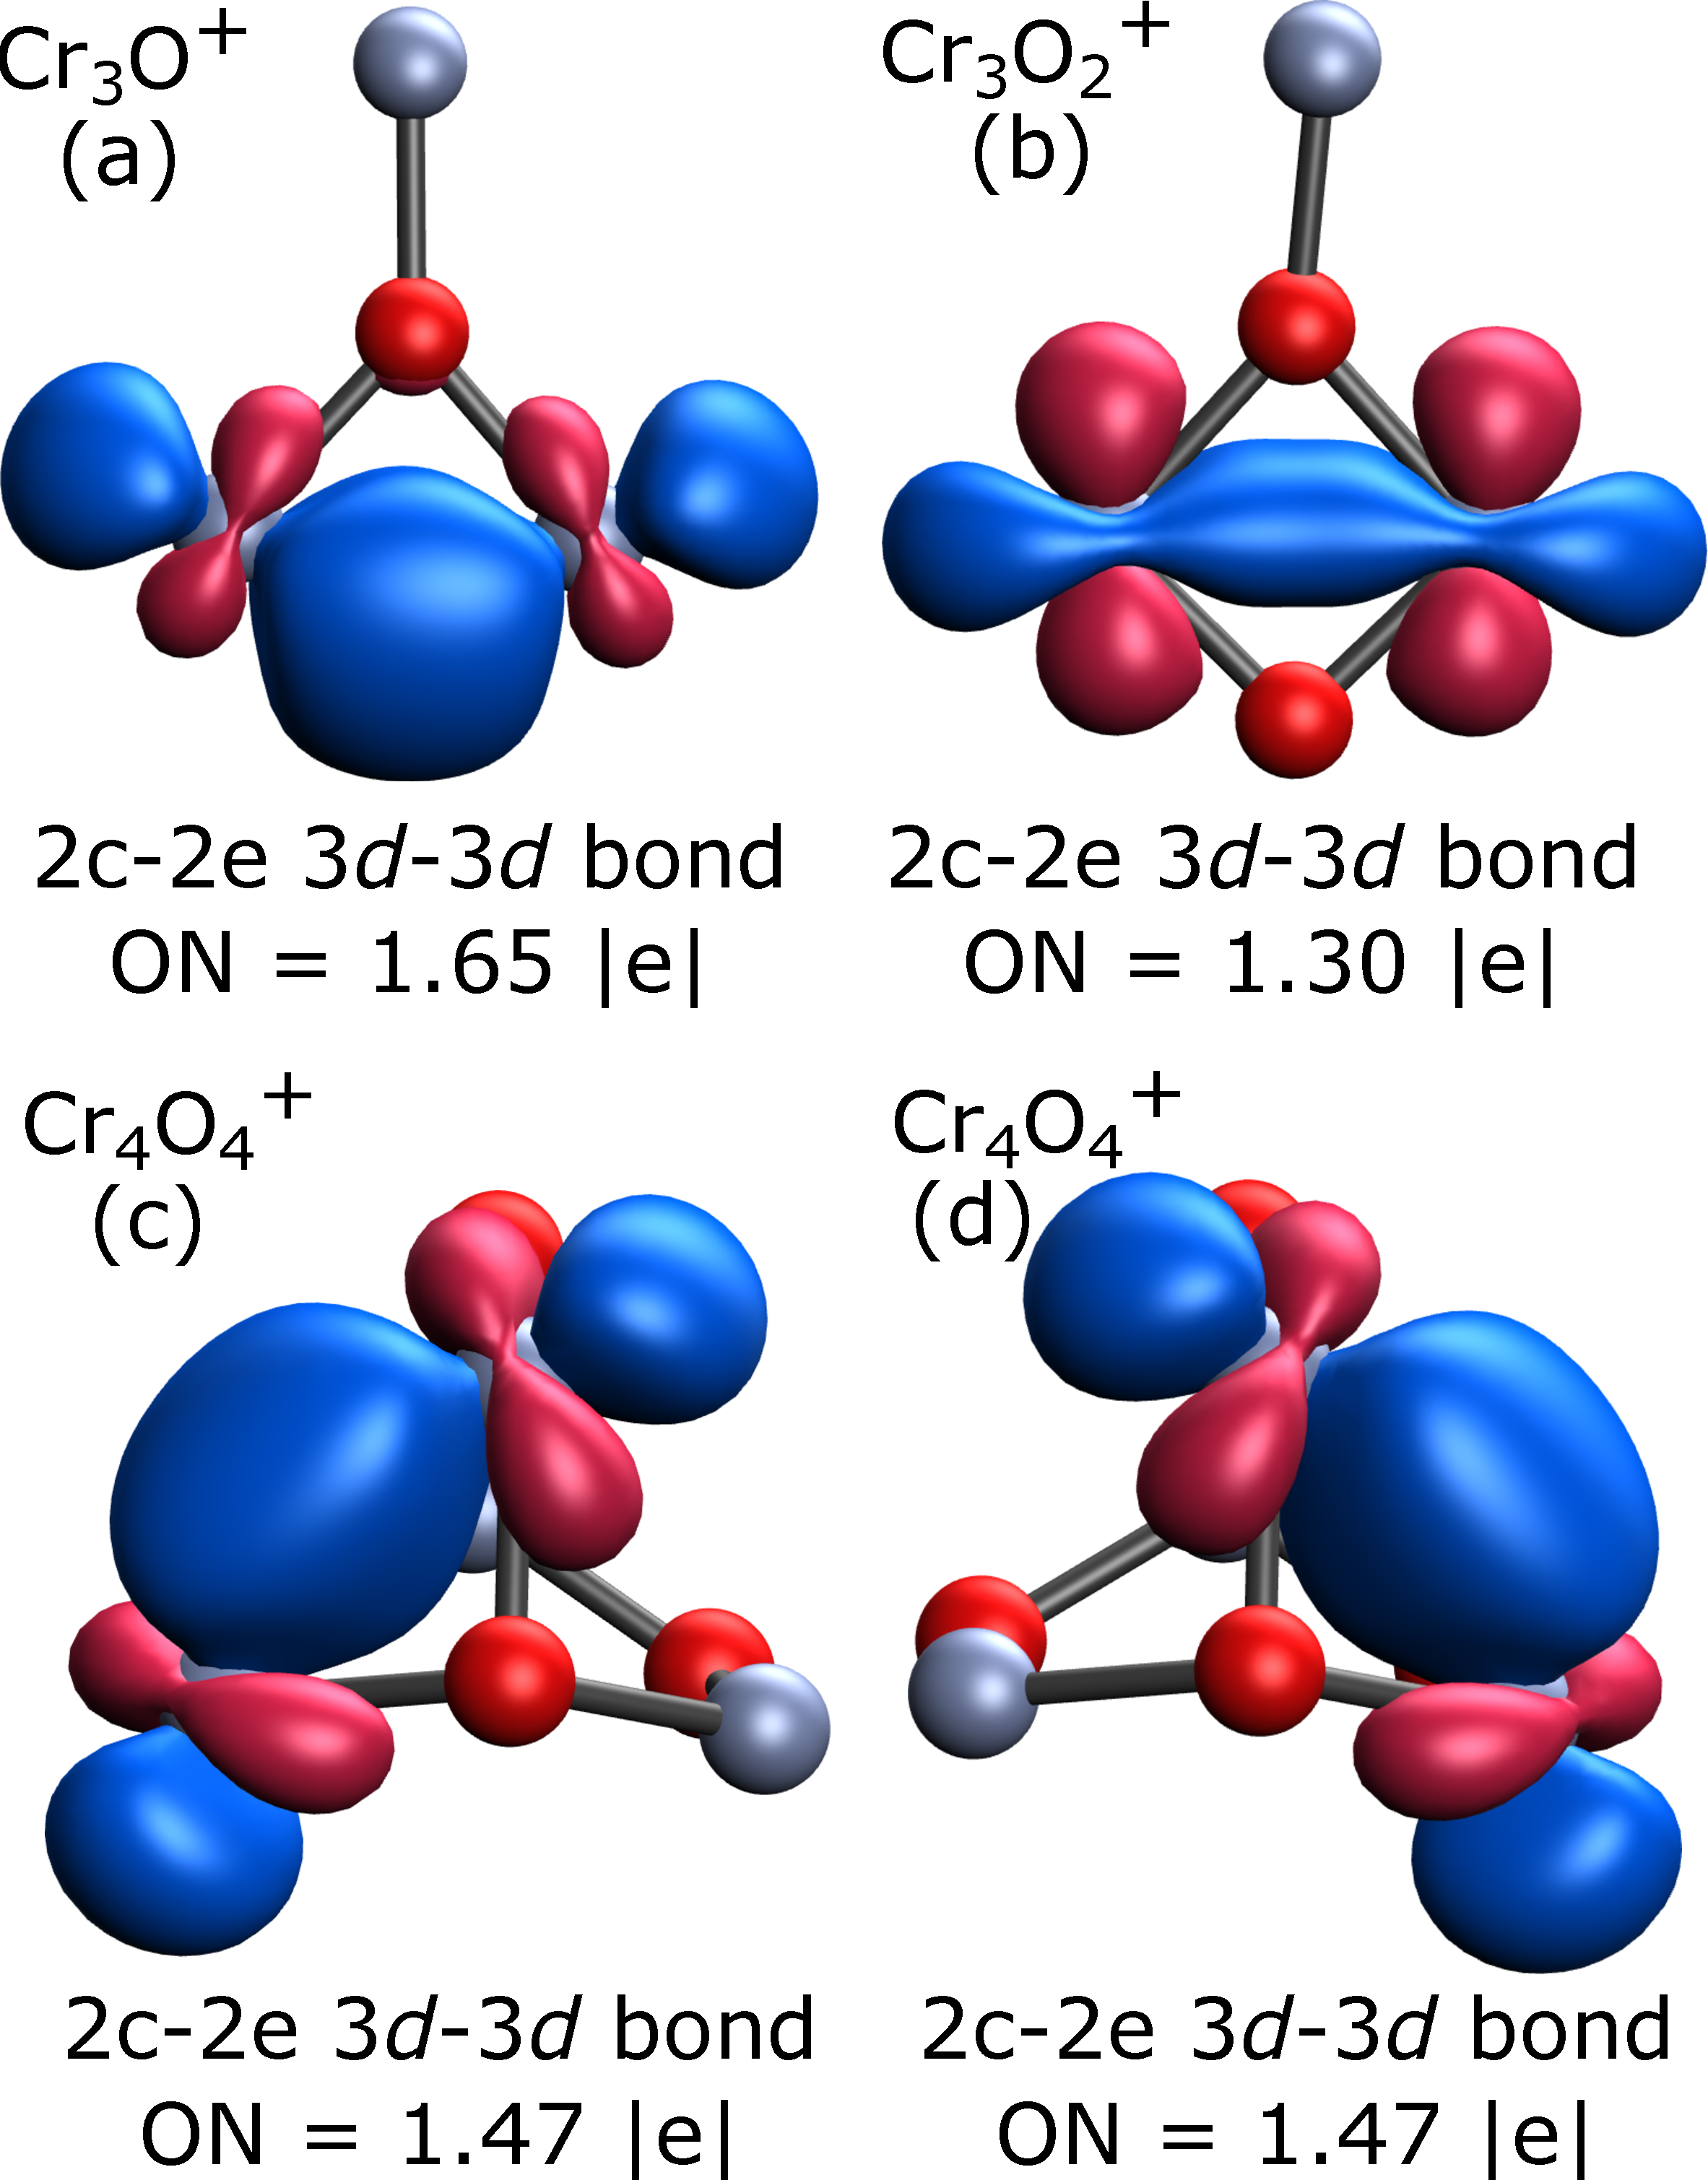
\includegraphics[width=0.4\textwidth]{AdNDP.pdf}
	\caption{2-center AdNDP bonding-type formation between two closer chromium atoms. 2-center bonds with largest occupation numbers are selected and plotted. Only chromium oxides with available experimental \acrshort{irpd}  spectra were analyzed.}
	\label{a7fig:AdNDP}
\end{figure}

Only 2-center metallic bonds with largest occupation numbers are selected. These 2-center bonding-like features depicted in Figure \ref{a7fig:AdNDP} are  weaker than normal 2-center 2-electron bondings because the occupation numbers of these AdNDP orbitals are around 1.5 (lesser than 2). The selection of 2-center bonds are on the basis of Cr-3d \acrshort{pdos} in Figure \ref{a7fig:dos} and Figure 6 where energetic overlap between alpha and beta 3d occupied orbitals of the two closest chromium atoms is found.

\newpage
\section{Density of states of \ce{C\lowercase{r}2O2+}, \ce{C\lowercase{r}3O2+} and \ce{C\lowercase{r}4O4+} }

\begin{figure}[ht]
    \centering
	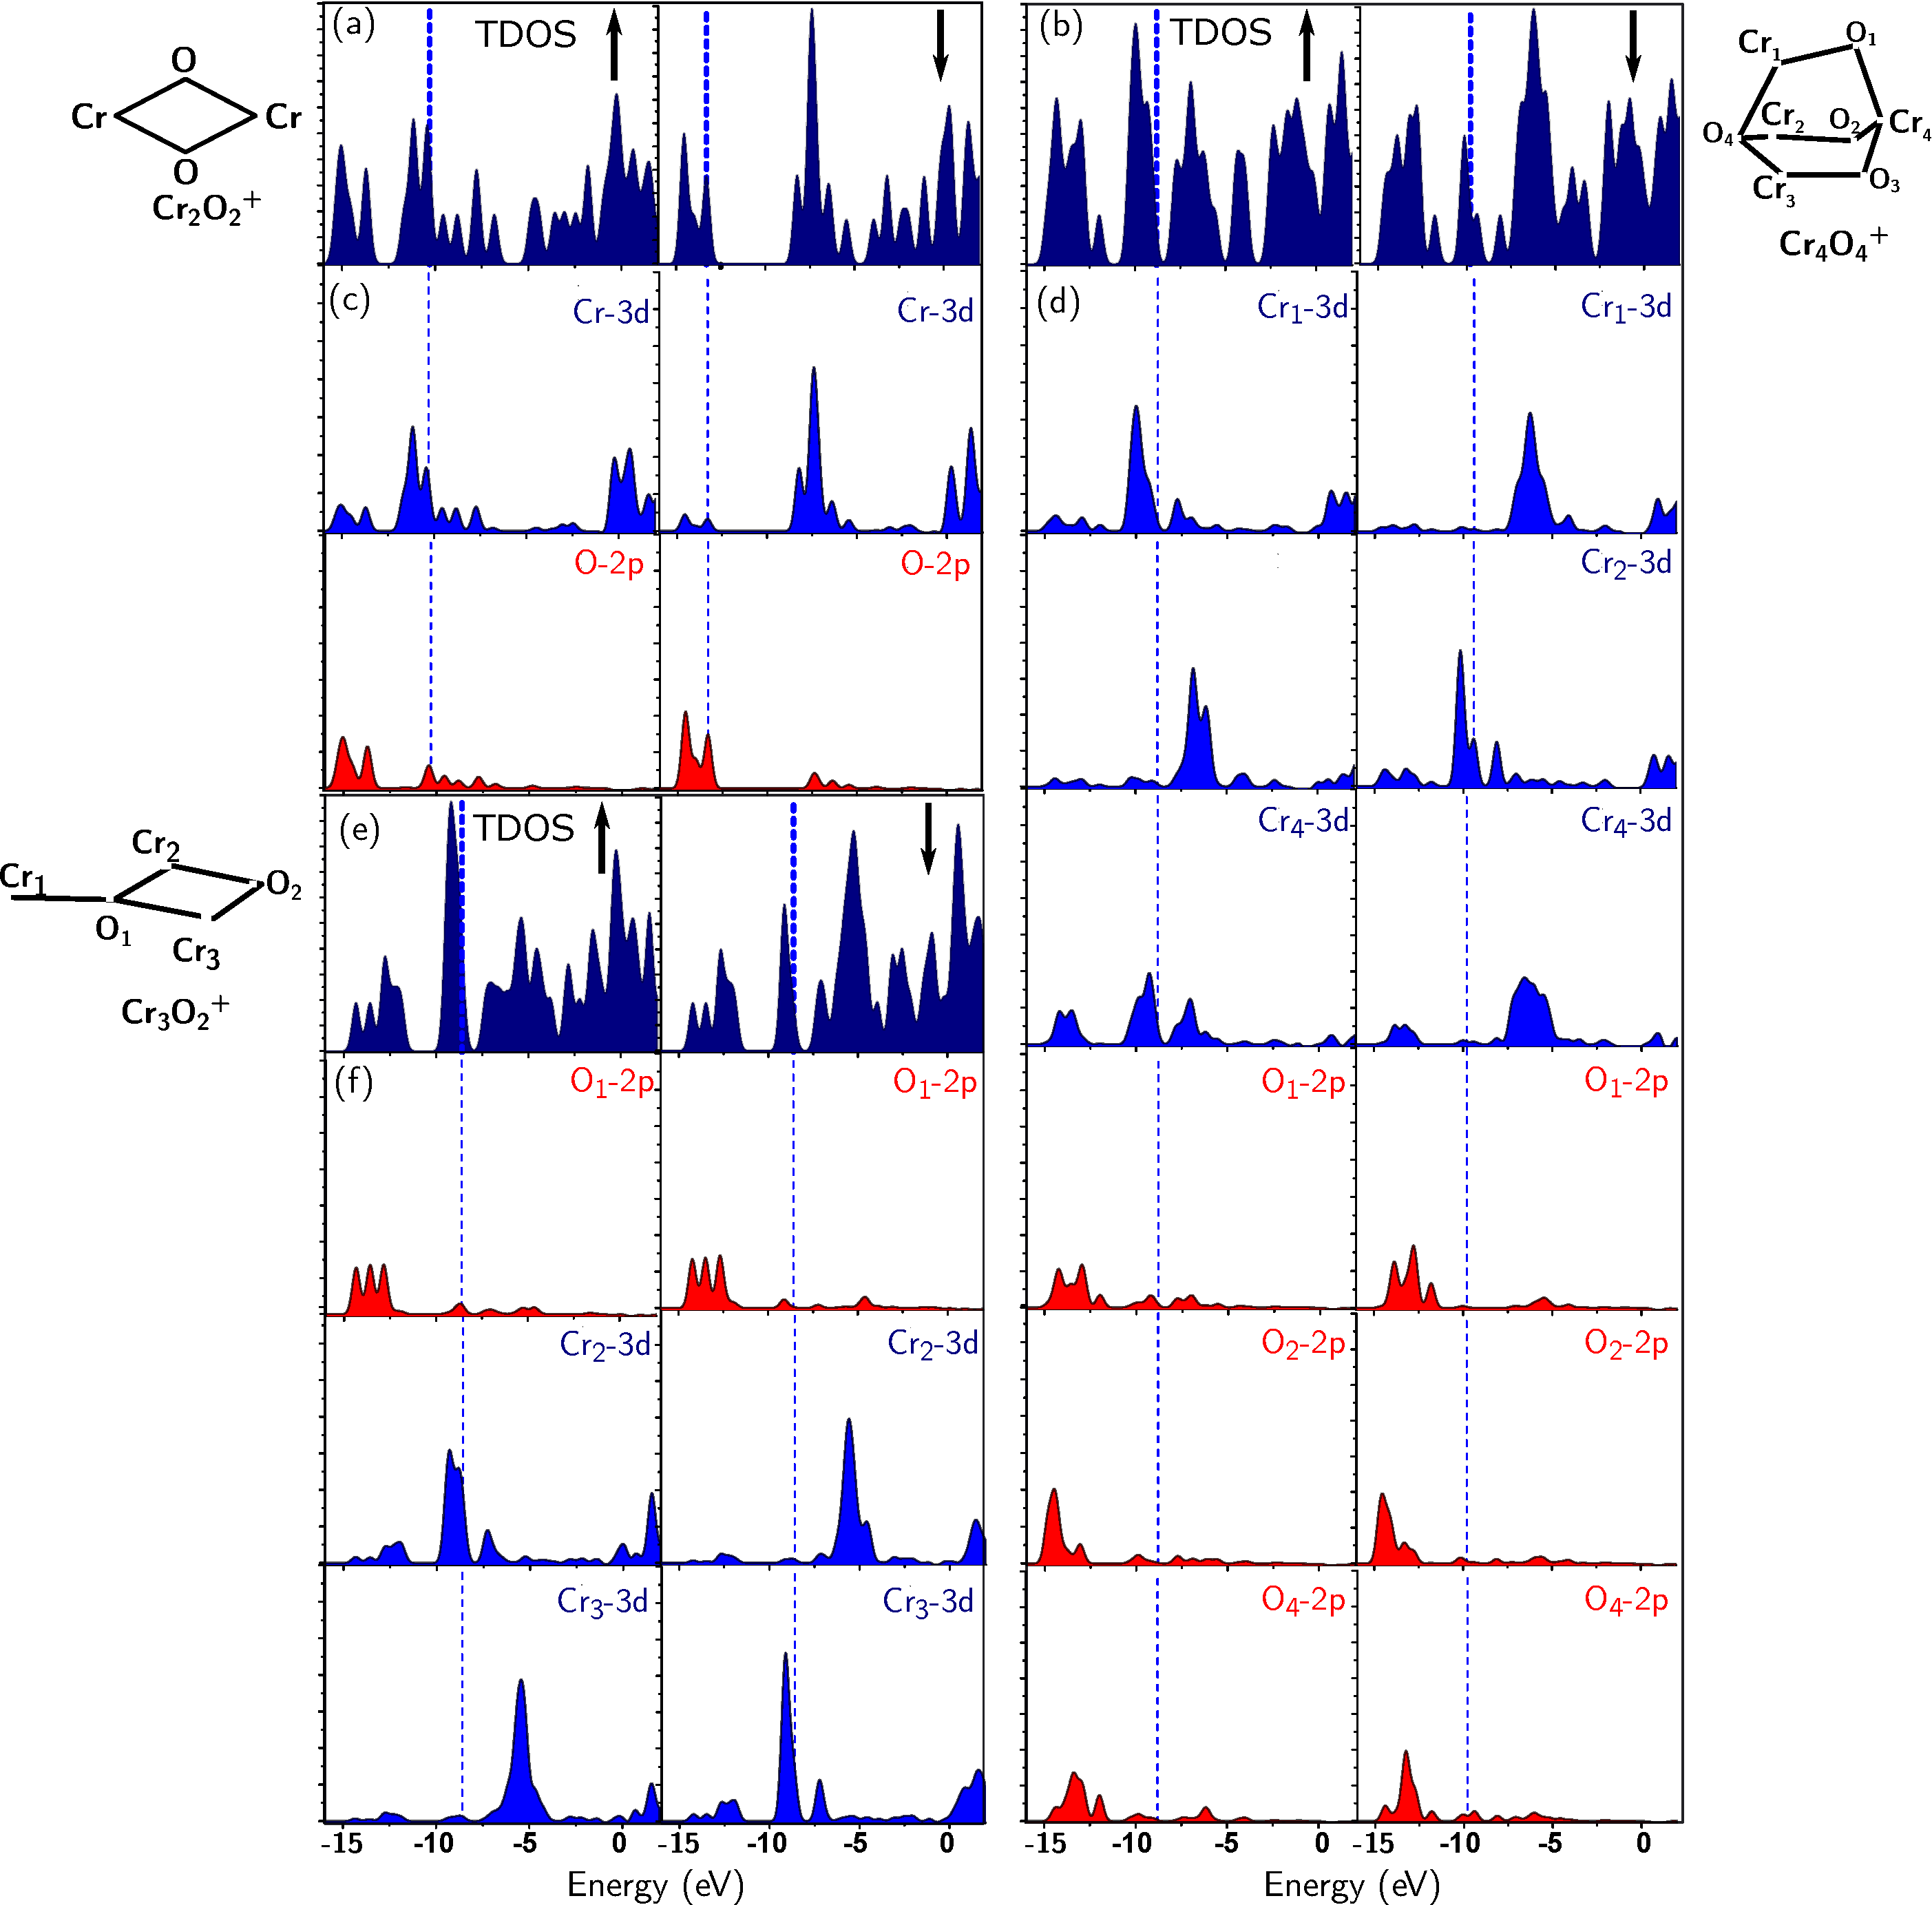
\includegraphics[width=0.91\textwidth]{DOS-SI.pdf}
	\caption{\acrshort{tdos} and \acrshort{pdos} of \ce{Cr2O2+} (top left), \ce{Cr3O2+} (bottom left) and \ce{Cr4O4+} (right). For each part the left (right) side corresponds to alpha (beta) orbitals as indicated by the black arrows. (a) \acrshort{tdos} of \ce{Cr2O2+}, (b) \acrshort{tdos} of \ce{Cr4O4+}, (c) \acrshort{pdos} of \ce{Cr2O2+}, (d) \acrshort{pdos} of \ce{Cr4O4+}, (e) \acrshort{tdos} of \ce{Cr3O2+}, and (f) \acrshort{pdos} of \ce{Cr3O2+}. \acrshort{pdos} projections in O-2p (Cr-3d) orbitals are shown in red (blue). Dashed lines indicate the \acrshort{homo} level.} 
	\label{a7fig:dos}
\end{figure}




















\cleardoublepage

\includebibliography
\printbibliography[heading=subbibliography] % print section bibliography

\end{refsection}


